\documentclass[twoside]{book}

% Packages required by doxygen
\usepackage{fixltx2e}
\usepackage{calc}
\usepackage{doxygen}
\usepackage[export]{adjustbox} % also loads graphicx
\usepackage{graphicx}
\usepackage[utf8]{inputenc}
\usepackage{makeidx}
\usepackage{multicol}
\usepackage{multirow}
\PassOptionsToPackage{warn}{textcomp}
\usepackage{textcomp}
\usepackage[nointegrals]{wasysym}
\usepackage[table]{xcolor}

% Font selection
\usepackage[T1]{fontenc}
\usepackage[scaled=.90]{helvet}
\usepackage{courier}
\usepackage{amssymb}
\usepackage{sectsty}
\renewcommand{\familydefault}{\sfdefault}
\allsectionsfont{%
  \fontseries{bc}\selectfont%
  \color{darkgray}%
}
\renewcommand{\DoxyLabelFont}{%
  \fontseries{bc}\selectfont%
  \color{darkgray}%
}
\newcommand{\+}{\discretionary{\mbox{\scriptsize$\hookleftarrow$}}{}{}}

% Page & text layout
\usepackage{geometry}
\geometry{%
  a4paper,%
  top=2.5cm,%
  bottom=2.5cm,%
  left=2.5cm,%
  right=2.5cm%
}
\tolerance=750
\hfuzz=15pt
\hbadness=750
\setlength{\emergencystretch}{15pt}
\setlength{\parindent}{0cm}
\setlength{\parskip}{3ex plus 2ex minus 2ex}
\makeatletter
\renewcommand{\paragraph}{%
  \@startsection{paragraph}{4}{0ex}{-1.0ex}{1.0ex}{%
    \normalfont\normalsize\bfseries\SS@parafont%
  }%
}
\renewcommand{\subparagraph}{%
  \@startsection{subparagraph}{5}{0ex}{-1.0ex}{1.0ex}{%
    \normalfont\normalsize\bfseries\SS@subparafont%
  }%
}
\makeatother

% Headers & footers
\usepackage{fancyhdr}
\pagestyle{fancyplain}
\fancyhead[LE]{\fancyplain{}{\bfseries\thepage}}
\fancyhead[CE]{\fancyplain{}{}}
\fancyhead[RE]{\fancyplain{}{\bfseries\leftmark}}
\fancyhead[LO]{\fancyplain{}{\bfseries\rightmark}}
\fancyhead[CO]{\fancyplain{}{}}
\fancyhead[RO]{\fancyplain{}{\bfseries\thepage}}
\fancyfoot[LE]{\fancyplain{}{}}
\fancyfoot[CE]{\fancyplain{}{}}
\fancyfoot[RE]{\fancyplain{}{\bfseries\scriptsize Generated by Doxygen }}
\fancyfoot[LO]{\fancyplain{}{\bfseries\scriptsize Generated by Doxygen }}
\fancyfoot[CO]{\fancyplain{}{}}
\fancyfoot[RO]{\fancyplain{}{}}
\renewcommand{\footrulewidth}{0.4pt}
\renewcommand{\chaptermark}[1]{%
  \markboth{#1}{}%
}
\renewcommand{\sectionmark}[1]{%
  \markright{\thesection\ #1}%
}

% Indices & bibliography
\usepackage{natbib}
\usepackage[titles]{tocloft}
\setcounter{tocdepth}{3}
\setcounter{secnumdepth}{5}
\makeindex

% Hyperlinks (required, but should be loaded last)
\usepackage{ifpdf}
\ifpdf
  \usepackage[pdftex,pagebackref=true]{hyperref}
\else
  \usepackage[ps2pdf,pagebackref=true]{hyperref}
\fi
\hypersetup{%
  colorlinks=true,%
  linkcolor=blue,%
  citecolor=blue,%
  unicode%
}

% Custom commands
\newcommand{\clearemptydoublepage}{%
  \newpage{\pagestyle{empty}\cleardoublepage}%
}

\usepackage{caption}
\captionsetup{labelsep=space,justification=centering,font={bf},singlelinecheck=off,skip=4pt,position=top}

%===== C O N T E N T S =====

\begin{document}

% Titlepage & ToC
\hypersetup{pageanchor=false,
             bookmarksnumbered=true,
             pdfencoding=unicode
            }
\pagenumbering{alph}
\begin{titlepage}
\vspace*{7cm}
\begin{center}%
{\Large Grande\+Omega Visualization }\\
\vspace*{1cm}
{\large Generated by Doxygen 1.8.14}\\
\end{center}
\end{titlepage}
\clearemptydoublepage
\pagenumbering{roman}
\tableofcontents
\clearemptydoublepage
\pagenumbering{arabic}
\hypersetup{pageanchor=true}

%--- Begin generated contents ---
\chapter{Hierarchical Index}
\section{Class Hierarchy}
This inheritance list is sorted roughly, but not completely, alphabetically\+:\begin{DoxyCompactList}
\item \contentsline{section}{Centroid}{\pageref{structCentroid}}{}
\item \contentsline{section}{Csv\+Parser}{\pageref{classCsvParser}}{}
\item \contentsline{section}{Database\+Interacter}{\pageref{classDatabaseInteracter}}{}
\item \contentsline{section}{D\+B\+S\+C\+AN}{\pageref{classDBSCAN}}{}
\item \contentsline{section}{Filter\+Context}{\pageref{structFilterContext}}{}
\item \contentsline{section}{Filter\+Query\+Column\+Indexes}{\pageref{structFilterQueryColumnIndexes}}{}
\item \contentsline{section}{Generic\+Vector}{\pageref{classGenericVector}}{}
\item \contentsline{section}{I\+Classifier}{\pageref{classIClassifier}}{}
\begin{DoxyCompactList}
\item \contentsline{section}{K\+Nearest\+Neighbours}{\pageref{classKNearestNeighbours}}{}
\item \contentsline{section}{Naive\+Bayes\+Classification}{\pageref{classNaiveBayesClassification}}{}
\end{DoxyCompactList}
\item \contentsline{section}{I\+Clustering\+Point}{\pageref{classIClusteringPoint}}{}
\begin{DoxyCompactList}
\item \contentsline{section}{D\+B\+Scan\+Point}{\pageref{classDBScanPoint}}{}
\item \contentsline{section}{K\+Means\+Point}{\pageref{classKMeansPoint}}{}
\end{DoxyCompactList}
\item \contentsline{section}{I\+Filter}{\pageref{classIFilter}}{}
\begin{DoxyCompactList}
\item \contentsline{section}{Assignment\+Interval\+Filter}{\pageref{classAssignmentIntervalFilter}}{}
\item \contentsline{section}{Grade\+Percentage\+Filter}{\pageref{classGradePercentageFilter}}{}
\item \contentsline{section}{I\+Time\+Filter}{\pageref{classITimeFilter}}{}
\begin{DoxyCompactList}
\item \contentsline{section}{Day\+Only\+Filter}{\pageref{classDayOnlyFilter}}{}
\item \contentsline{section}{Night\+Only\+Filter}{\pageref{classNightOnlyFilter}}{}
\item \contentsline{section}{Week\+Day\+Filter}{\pageref{classWeekDayFilter}}{}
\item \contentsline{section}{Weekend\+Day\+Filter}{\pageref{classWeekendDayFilter}}{}
\end{DoxyCompactList}
\end{DoxyCompactList}
\item \contentsline{section}{I\+Regression}{\pageref{classIRegression}}{}
\begin{DoxyCompactList}
\item \contentsline{section}{Logarithmic\+Linear\+Regression}{\pageref{classLogarithmicLinearRegression}}{}
\item \contentsline{section}{Simple\+Linear\+Regression}{\pageref{classSimpleLinearRegression}}{}
\end{DoxyCompactList}
\item \contentsline{section}{I\+Visualization}{\pageref{classIVisualization}}{}
\begin{DoxyCompactList}
\item \contentsline{section}{Amount\+Of\+Students\+Per\+Class}{\pageref{classAmountOfStudentsPerClass}}{}
\item \contentsline{section}{Correlation\+Measures}{\pageref{classCorrelationMeasures}}{}
\item \contentsline{section}{Excersise\+Completion\+And\+Grades\+Clustering}{\pageref{classExcersiseCompletionAndGradesClustering}}{}
\item \contentsline{section}{Grade\+And\+Excersise\+Successes}{\pageref{classGradeAndExcersiseSuccesses}}{}
\item \contentsline{section}{Grade\+Avgs\+Per\+Class}{\pageref{classGradeAvgsPerClass}}{}
\item \contentsline{section}{I\+Classification\+Visualization}{\pageref{classIClassificationVisualization}}{}
\begin{DoxyCompactList}
\item \contentsline{section}{Day\+Only\+Completions\+Vs\+Grade\+Classification}{\pageref{classDayOnlyCompletionsVsGradeClassification}}{}
\item \contentsline{section}{Night\+Only\+Completions\+Vs\+Grade\+Classification}{\pageref{classNightOnlyCompletionsVsGradeClassification}}{}
\item \contentsline{section}{Week\+Day\+Excersise\+Completion\+And\+Grades\+Classification}{\pageref{classWeekDayExcersiseCompletionAndGradesClassification}}{}
\end{DoxyCompactList}
\end{DoxyCompactList}
\item \contentsline{section}{J\+S\+O\+N\+Encoder}{\pageref{classJSONEncoder}}{}
\item \contentsline{section}{K\+Means\+Controller}{\pageref{classKMeansController}}{}
\item \contentsline{section}{K\+Means\+Iteration}{\pageref{classKMeansIteration}}{}
\item \contentsline{section}{Mapper}{\pageref{classMapper}}{}
\item Test\+Fixture\begin{DoxyCompactList}
\item \contentsline{section}{Simple\+Linear\+Regression\+Test}{\pageref{classSimpleLinearRegressionTest}}{}
\item \contentsline{section}{Statistical\+Tools\+Test}{\pageref{classStatisticalToolsTest}}{}
\item \contentsline{section}{Utilities\+Test}{\pageref{classUtilitiesTest}}{}
\end{DoxyCompactList}
\item \contentsline{section}{Utc\+Reader}{\pageref{classUtcReader}}{}
\item \contentsline{section}{Utc\+Time}{\pageref{classUtcTime}}{}
\item \contentsline{section}{Utilities}{\pageref{classUtilities}}{}
\item \contentsline{section}{Yaml\+Converter}{\pageref{classYamlConverter}}{}
\item \contentsline{section}{Yaml\+Object}{\pageref{classYamlObject}}{}
\item \contentsline{section}{Yaml\+Parser}{\pageref{classYamlParser}}{}
\end{DoxyCompactList}

\chapter{Class Index}
\section{Class List}
Here are the classes, structs, unions and interfaces with brief descriptions\+:\begin{DoxyCompactList}
\item\contentsline{section}{\hyperlink{classAmountOfStudentsPerClass}{Amount\+Of\+Students\+Per\+Class} }{\pageref{classAmountOfStudentsPerClass}}{}
\item\contentsline{section}{\hyperlink{classAssignmentIntervalFilter}{Assignment\+Interval\+Filter} }{\pageref{classAssignmentIntervalFilter}}{}
\item\contentsline{section}{\hyperlink{structCentroid}{Centroid} }{\pageref{structCentroid}}{}
\item\contentsline{section}{\hyperlink{classCorrelationMeasures}{Correlation\+Measures} }{\pageref{classCorrelationMeasures}}{}
\item\contentsline{section}{\hyperlink{classCsvParser}{Csv\+Parser} }{\pageref{classCsvParser}}{}
\item\contentsline{section}{\hyperlink{classDatabaseInteracter}{Database\+Interacter} }{\pageref{classDatabaseInteracter}}{}
\item\contentsline{section}{\hyperlink{classDayOnlyCompletionsVsGradeClassification}{Day\+Only\+Completions\+Vs\+Grade\+Classification} }{\pageref{classDayOnlyCompletionsVsGradeClassification}}{}
\item\contentsline{section}{\hyperlink{classDayOnlyFilter}{Day\+Only\+Filter} }{\pageref{classDayOnlyFilter}}{}
\item\contentsline{section}{\hyperlink{classDBSCAN}{D\+B\+S\+C\+AN} }{\pageref{classDBSCAN}}{}
\item\contentsline{section}{\hyperlink{classDBScanPoint}{D\+B\+Scan\+Point} }{\pageref{classDBScanPoint}}{}
\item\contentsline{section}{\hyperlink{classExcersiseCompletionAndGradesClustering}{Excersise\+Completion\+And\+Grades\+Clustering} }{\pageref{classExcersiseCompletionAndGradesClustering}}{}
\item\contentsline{section}{\hyperlink{structFilterContext}{Filter\+Context} }{\pageref{structFilterContext}}{}
\item\contentsline{section}{\hyperlink{structFilterQueryColumnIndexes}{Filter\+Query\+Column\+Indexes} }{\pageref{structFilterQueryColumnIndexes}}{}
\item\contentsline{section}{\hyperlink{classGenericVector}{Generic\+Vector} }{\pageref{classGenericVector}}{}
\item\contentsline{section}{\hyperlink{classGradeAndExcersiseSuccesses}{Grade\+And\+Excersise\+Successes} }{\pageref{classGradeAndExcersiseSuccesses}}{}
\item\contentsline{section}{\hyperlink{classGradeAvgsPerClass}{Grade\+Avgs\+Per\+Class} }{\pageref{classGradeAvgsPerClass}}{}
\item\contentsline{section}{\hyperlink{classGradePercentageFilter}{Grade\+Percentage\+Filter} }{\pageref{classGradePercentageFilter}}{}
\item\contentsline{section}{\hyperlink{classIClassificationVisualization}{I\+Classification\+Visualization} }{\pageref{classIClassificationVisualization}}{}
\item\contentsline{section}{\hyperlink{classIClassifier}{I\+Classifier} }{\pageref{classIClassifier}}{}
\item\contentsline{section}{\hyperlink{classIClusteringPoint}{I\+Clustering\+Point} }{\pageref{classIClusteringPoint}}{}
\item\contentsline{section}{\hyperlink{classIFilter}{I\+Filter} }{\pageref{classIFilter}}{}
\item\contentsline{section}{\hyperlink{classIRegression}{I\+Regression} }{\pageref{classIRegression}}{}
\item\contentsline{section}{\hyperlink{classITimeFilter}{I\+Time\+Filter} }{\pageref{classITimeFilter}}{}
\item\contentsline{section}{\hyperlink{classIVisualization}{I\+Visualization} }{\pageref{classIVisualization}}{}
\item\contentsline{section}{\hyperlink{classJSONEncoder}{J\+S\+O\+N\+Encoder} }{\pageref{classJSONEncoder}}{}
\item\contentsline{section}{\hyperlink{classKMeansController}{K\+Means\+Controller} }{\pageref{classKMeansController}}{}
\item\contentsline{section}{\hyperlink{classKMeansIteration}{K\+Means\+Iteration} }{\pageref{classKMeansIteration}}{}
\item\contentsline{section}{\hyperlink{classKMeansPoint}{K\+Means\+Point} }{\pageref{classKMeansPoint}}{}
\item\contentsline{section}{\hyperlink{classKNearestNeighbours}{K\+Nearest\+Neighbours} }{\pageref{classKNearestNeighbours}}{}
\item\contentsline{section}{\hyperlink{classLogarithmicLinearRegression}{Logarithmic\+Linear\+Regression} }{\pageref{classLogarithmicLinearRegression}}{}
\item\contentsline{section}{\hyperlink{classMapper}{Mapper} }{\pageref{classMapper}}{}
\item\contentsline{section}{\hyperlink{classNaiveBayesClassification}{Naive\+Bayes\+Classification} }{\pageref{classNaiveBayesClassification}}{}
\item\contentsline{section}{\hyperlink{classNightOnlyCompletionsVsGradeClassification}{Night\+Only\+Completions\+Vs\+Grade\+Classification} }{\pageref{classNightOnlyCompletionsVsGradeClassification}}{}
\item\contentsline{section}{\hyperlink{classNightOnlyFilter}{Night\+Only\+Filter} }{\pageref{classNightOnlyFilter}}{}
\item\contentsline{section}{\hyperlink{classSimpleLinearRegression}{Simple\+Linear\+Regression} }{\pageref{classSimpleLinearRegression}}{}
\item\contentsline{section}{\hyperlink{classSimpleLinearRegressionTest}{Simple\+Linear\+Regression\+Test} }{\pageref{classSimpleLinearRegressionTest}}{}
\item\contentsline{section}{\hyperlink{classStatisticalToolsTest}{Statistical\+Tools\+Test} }{\pageref{classStatisticalToolsTest}}{}
\item\contentsline{section}{\hyperlink{classUtcReader}{Utc\+Reader} }{\pageref{classUtcReader}}{}
\item\contentsline{section}{\hyperlink{classUtcTime}{Utc\+Time} }{\pageref{classUtcTime}}{}
\item\contentsline{section}{\hyperlink{classUtilities}{Utilities} }{\pageref{classUtilities}}{}
\item\contentsline{section}{\hyperlink{classUtilitiesTest}{Utilities\+Test} }{\pageref{classUtilitiesTest}}{}
\item\contentsline{section}{\hyperlink{classWeekDayExcersiseCompletionAndGradesClassification}{Week\+Day\+Excersise\+Completion\+And\+Grades\+Classification} }{\pageref{classWeekDayExcersiseCompletionAndGradesClassification}}{}
\item\contentsline{section}{\hyperlink{classWeekDayFilter}{Week\+Day\+Filter} }{\pageref{classWeekDayFilter}}{}
\item\contentsline{section}{\hyperlink{classWeekendDayFilter}{Weekend\+Day\+Filter} }{\pageref{classWeekendDayFilter}}{}
\item\contentsline{section}{\hyperlink{classYamlConverter}{Yaml\+Converter} }{\pageref{classYamlConverter}}{}
\item\contentsline{section}{\hyperlink{classYamlObject}{Yaml\+Object} }{\pageref{classYamlObject}}{}
\item\contentsline{section}{\hyperlink{classYamlParser}{Yaml\+Parser} }{\pageref{classYamlParser}}{}
\end{DoxyCompactList}

\chapter{Class Documentation}
\hypertarget{classAmountOfStudentsPerClass}{}\section{Amount\+Of\+Students\+Per\+Class Class Reference}
\label{classAmountOfStudentsPerClass}\index{Amount\+Of\+Students\+Per\+Class@{Amount\+Of\+Students\+Per\+Class}}
Inheritance diagram for Amount\+Of\+Students\+Per\+Class\+:\begin{figure}[H]
\begin{center}
\leavevmode
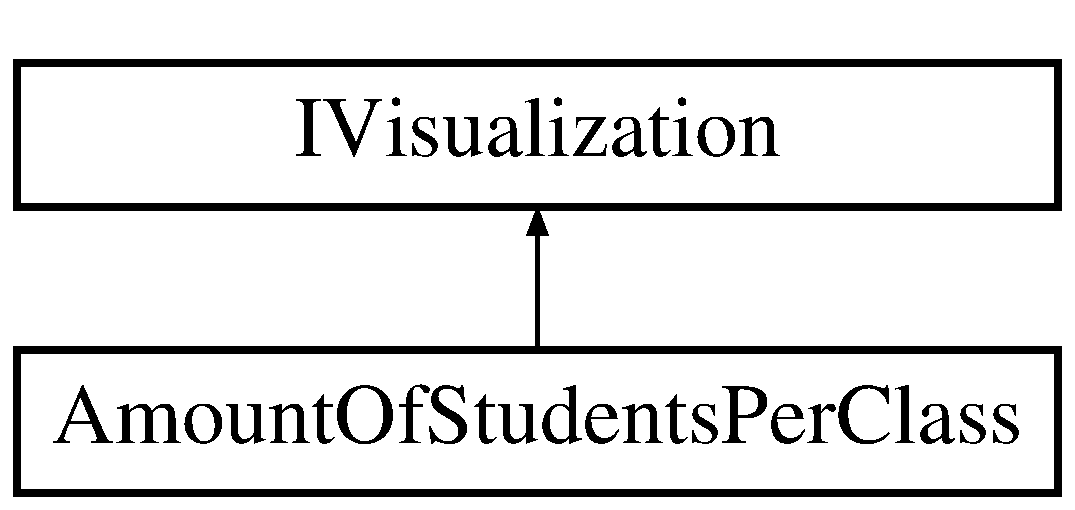
\includegraphics[height=2.000000cm]{classAmountOfStudentsPerClass}
\end{center}
\end{figure}
\subsection*{Public Member Functions}
\begin{DoxyCompactItemize}
\item 
\mbox{\Hypertarget{classAmountOfStudentsPerClass_a77700a31cecd7c30bcc1637b7f909f78}\label{classAmountOfStudentsPerClass_a77700a31cecd7c30bcc1637b7f909f78}} 
std\+::string {\bfseries get\+Visualization\+As\+J\+S\+ON} ()
\end{DoxyCompactItemize}


The documentation for this class was generated from the following files\+:\begin{DoxyCompactItemize}
\item 
Data\+Processer/src/\+Statistical\+Analyzer/\+Visualizations/Amount\+Of\+Students\+Per\+Class.\+h\item 
Data\+Processer/src/\+Statistical\+Analyzer/\+Visualizations/Amount\+Of\+Students\+Per\+Class.\+cpp\end{DoxyCompactItemize}

\hypertarget{classAssignmentIntervalFilter}{}\section{Assignment\+Interval\+Filter Class Reference}
\label{classAssignmentIntervalFilter}\index{Assignment\+Interval\+Filter@{Assignment\+Interval\+Filter}}
Inheritance diagram for Assignment\+Interval\+Filter\+:\begin{figure}[H]
\begin{center}
\leavevmode
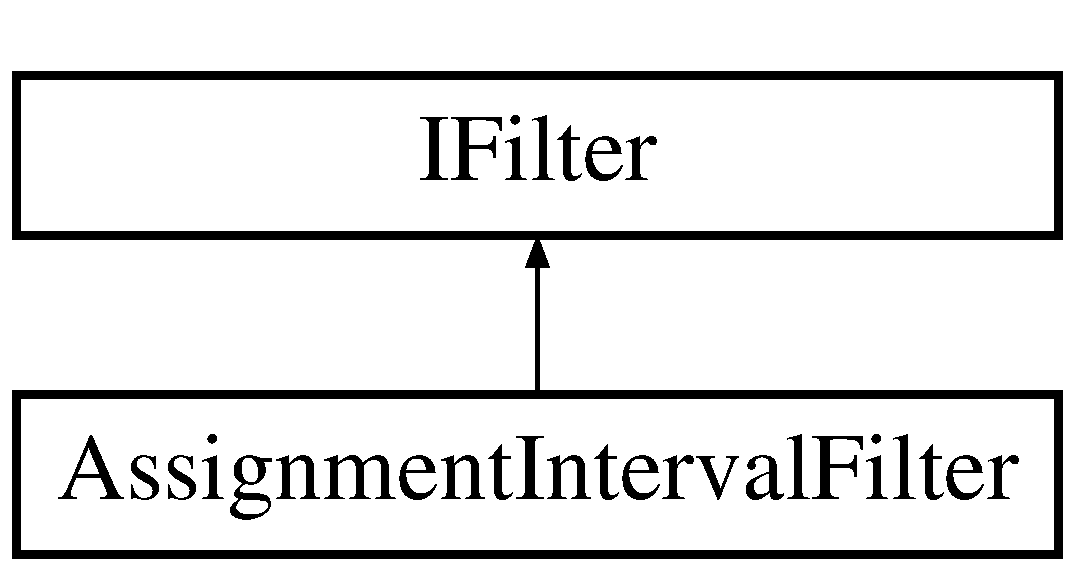
\includegraphics[height=2.000000cm]{classAssignmentIntervalFilter}
\end{center}
\end{figure}
\subsection*{Public Member Functions}
\begin{DoxyCompactItemize}
\item 
\mbox{\Hypertarget{classAssignmentIntervalFilter_a7763deed2ff29d0b97ee2648e4c7a87a}\label{classAssignmentIntervalFilter_a7763deed2ff29d0b97ee2648e4c7a87a}} 
void {\bfseries set\+Filter\+Query\+Column\+Indexes} (\hyperlink{structFilterQueryColumnIndexes}{Filter\+Query\+Column\+Indexes} fq)
\item 
\mbox{\Hypertarget{classAssignmentIntervalFilter_acda0705d8c1e9a28c7a0808b3dd5e26e}\label{classAssignmentIntervalFilter_acda0705d8c1e9a28c7a0808b3dd5e26e}} 
\hyperlink{structFilterQueryColumnIndexes}{Filter\+Query\+Column\+Indexes} {\bfseries get\+Filter\+Query\+Column\+Indexes} ()
\item 
\mbox{\Hypertarget{classAssignmentIntervalFilter_a8c287c27d918c3aa708b6f46cba11a90}\label{classAssignmentIntervalFilter_a8c287c27d918c3aa708b6f46cba11a90}} 
void {\bfseries set\+Filter\+Context} (\hyperlink{structFilterContext}{Filter\+Context} fc)
\item 
\mbox{\Hypertarget{classAssignmentIntervalFilter_a038d995082af531cc9c650c08cd1224e}\label{classAssignmentIntervalFilter_a038d995082af531cc9c650c08cd1224e}} 
\hyperlink{structFilterContext}{Filter\+Context} {\bfseries get\+Filter\+Context} ()
\item 
\mbox{\Hypertarget{classAssignmentIntervalFilter_a9013b1e23261151e22aa4b78980f5279}\label{classAssignmentIntervalFilter_a9013b1e23261151e22aa4b78980f5279}} 
std\+::vector$<$ pqxx\+::result\+::tuple $>$ {\bfseries filter} (std\+::vector$<$ pqxx\+::result\+::tuple $>$ unfiltered\+Rows)
\item 
\mbox{\Hypertarget{classAssignmentIntervalFilter_a74be4426b988fcbde79e7b6b181e567d}\label{classAssignmentIntervalFilter_a74be4426b988fcbde79e7b6b181e567d}} 
{\bfseries Assignment\+Interval\+Filter} (\hyperlink{structFilterContext}{Filter\+Context} f)
\end{DoxyCompactItemize}
\subsection*{Public Attributes}
\begin{DoxyCompactItemize}
\item 
\mbox{\Hypertarget{classAssignmentIntervalFilter_aadf2eaa2ab5e7bf8d620b2baacaf5d16}\label{classAssignmentIntervalFilter_aadf2eaa2ab5e7bf8d620b2baacaf5d16}} 
\hyperlink{structFilterQueryColumnIndexes}{Filter\+Query\+Column\+Indexes} {\bfseries query\+Column\+Indexes}
\item 
\mbox{\Hypertarget{classAssignmentIntervalFilter_a79a00626642f1b66af389e4e41f3aa83}\label{classAssignmentIntervalFilter_a79a00626642f1b66af389e4e41f3aa83}} 
\hyperlink{structFilterContext}{Filter\+Context} {\bfseries filter\+Context}
\end{DoxyCompactItemize}


The documentation for this class was generated from the following files\+:\begin{DoxyCompactItemize}
\item 
Data\+Processer/src/\+Statistical\+Analyzer/\+Filter/Assignment\+Interval\+Filter.\+h\item 
Data\+Processer/src/\+Statistical\+Analyzer/\+Filter/Assignment\+Interval\+Filter.\+cpp\end{DoxyCompactItemize}

\hypertarget{classAttemptsVsFailures}{}\section{Attempts\+Vs\+Failures Class Reference}
\label{classAttemptsVsFailures}\index{Attempts\+Vs\+Failures@{Attempts\+Vs\+Failures}}
Inheritance diagram for Attempts\+Vs\+Failures\+:\begin{figure}[H]
\begin{center}
\leavevmode
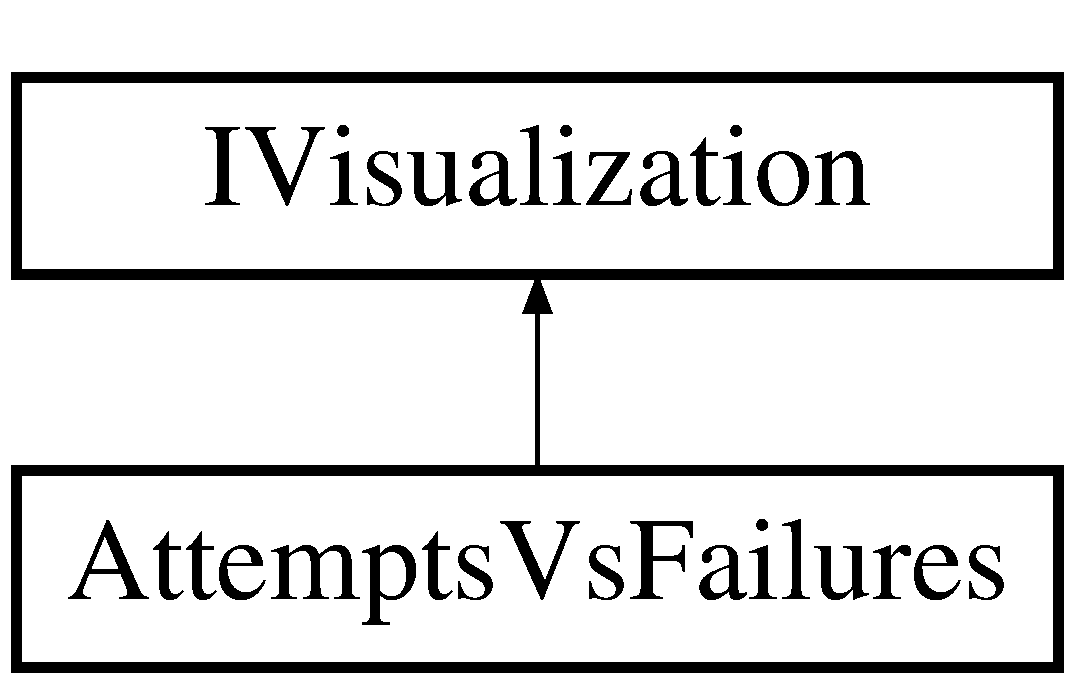
\includegraphics[height=2.000000cm]{classAttemptsVsFailures}
\end{center}
\end{figure}
\subsection*{Public Member Functions}
\begin{DoxyCompactItemize}
\item 
\mbox{\Hypertarget{classAttemptsVsFailures_ac8d34f57c579c66e96fc5d5a83397c5f}\label{classAttemptsVsFailures_ac8d34f57c579c66e96fc5d5a83397c5f}} 
std\+::string {\bfseries get\+Visualization\+As\+J\+S\+ON} ()
\end{DoxyCompactItemize}


The documentation for this class was generated from the following files\+:\begin{DoxyCompactItemize}
\item 
Data\+Processer/src/\+Statistical\+Analyzer/\+Visualizations/Attempts\+Vs\+Failures.\+h\item 
Data\+Processer/src/\+Statistical\+Analyzer/\+Visualizations/Attempts\+Vs\+Failures.\+cpp\end{DoxyCompactItemize}

\hypertarget{structCentroid}{}\section{Centroid Struct Reference}
\label{structCentroid}\index{Centroid@{Centroid}}
\subsection*{Public Member Functions}
\begin{DoxyCompactItemize}
\item 
\mbox{\Hypertarget{structCentroid_a62991a426ab204818dc692223af4aba0}\label{structCentroid_a62991a426ab204818dc692223af4aba0}} 
{\bfseries Centroid} (int i, \hyperlink{classGenericVector}{Generic\+Vector} gv)
\end{DoxyCompactItemize}
\subsection*{Public Attributes}
\begin{DoxyCompactItemize}
\item 
\mbox{\Hypertarget{structCentroid_a8856877441529189b74f69e3064e51e2}\label{structCentroid_a8856877441529189b74f69e3064e51e2}} 
int {\bfseries id}
\item 
\mbox{\Hypertarget{structCentroid_a3158c9ab870ec09dc2361231184d16f1}\label{structCentroid_a3158c9ab870ec09dc2361231184d16f1}} 
bool {\bfseries has\+Changed} = true
\item 
\mbox{\Hypertarget{structCentroid_a98847724eb23cac48cecd329f3b66c7e}\label{structCentroid_a98847724eb23cac48cecd329f3b66c7e}} 
\hyperlink{classGenericVector}{Generic\+Vector} {\bfseries vector}
\end{DoxyCompactItemize}


The documentation for this struct was generated from the following file\+:\begin{DoxyCompactItemize}
\item 
Data\+Processer/src/\+Statistical\+Analyzer/\+Point/K\+Means\+Point.\+h\end{DoxyCompactItemize}

\hypertarget{classCorrelationMeasures}{}\section{Correlation\+Measures Class Reference}
\label{classCorrelationMeasures}\index{Correlation\+Measures@{Correlation\+Measures}}
Inheritance diagram for Correlation\+Measures\+:\begin{figure}[H]
\begin{center}
\leavevmode
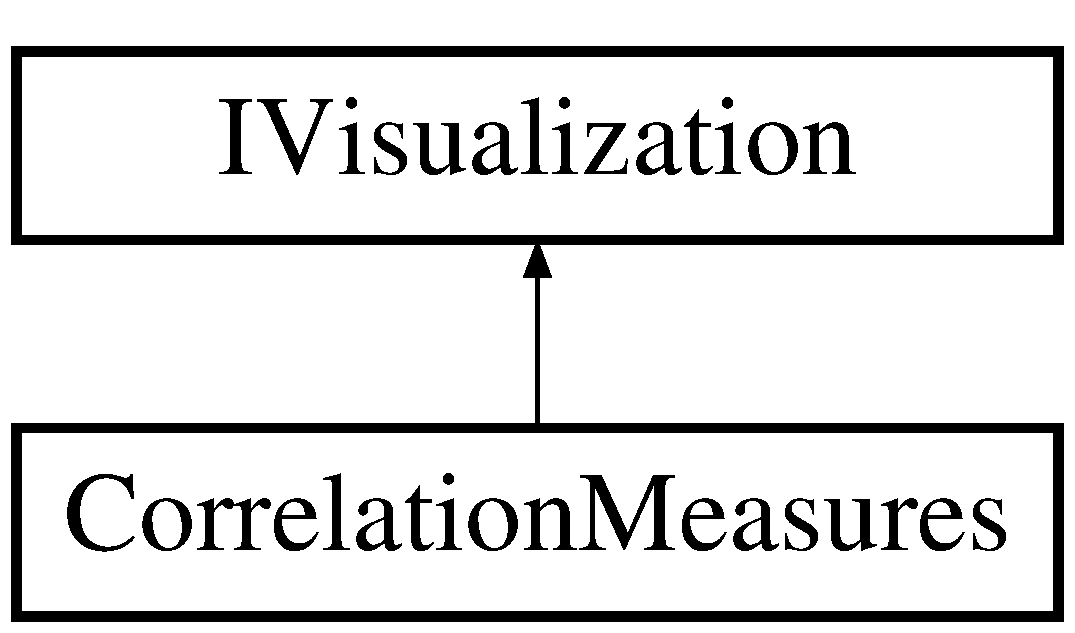
\includegraphics[height=2.000000cm]{classCorrelationMeasures}
\end{center}
\end{figure}
\subsection*{Public Member Functions}
\begin{DoxyCompactItemize}
\item 
\mbox{\Hypertarget{classCorrelationMeasures_ab51972b6029232bb8ddfa9f518ebd205}\label{classCorrelationMeasures_ab51972b6029232bb8ddfa9f518ebd205}} 
std\+::string {\bfseries get\+Visualization\+As\+J\+S\+ON} ()
\item 
\mbox{\Hypertarget{classCorrelationMeasures_aa9a5f39548be29db3fa7a7710691725b}\label{classCorrelationMeasures_aa9a5f39548be29db3fa7a7710691725b}} 
{\bfseries Correlation\+Measures} (std\+::pair$<$ \hyperlink{classGenericVector}{Generic\+Vector}, \hyperlink{classGenericVector}{Generic\+Vector} $>$ xy)
\end{DoxyCompactItemize}


The documentation for this class was generated from the following files\+:\begin{DoxyCompactItemize}
\item 
Data\+Processer/src/\+Statistical\+Analyzer/\+Visualizations/Correlation\+Measures.\+h\item 
Data\+Processer/src/\+Statistical\+Analyzer/\+Visualizations/Correlation\+Measures.\+cpp\end{DoxyCompactItemize}

\hypertarget{classCsvParser}{}\section{Csv\+Parser Class Reference}
\label{classCsvParser}\index{Csv\+Parser@{Csv\+Parser}}
\subsection*{Static Public Member Functions}
\begin{DoxyCompactItemize}
\item 
\mbox{\Hypertarget{classCsvParser_a6f7c94b8d8cdeaf79f913ffc5571d884}\label{classCsvParser_a6f7c94b8d8cdeaf79f913ffc5571d884}} 
static vector$<$ vector$<$ string $>$ $>$ {\bfseries parse\+Class\+Matrix} (ifstream \&str)
\item 
\mbox{\Hypertarget{classCsvParser_addbc1c755de70fa9e6366be186c43207}\label{classCsvParser_addbc1c755de70fa9e6366be186c43207}} 
static vector$<$ pair$<$ string, string $>$ $>$ {\bfseries parse\+Grade\+File} (ifstream \&str)
\end{DoxyCompactItemize}


The documentation for this class was generated from the following files\+:\begin{DoxyCompactItemize}
\item 
Data\+Processer/src/\+Csv\+Parser/Csv\+Parser.\+h\item 
Data\+Processer/src/\+Csv\+Parser/Csv\+Parser.\+cpp\end{DoxyCompactItemize}

\hypertarget{classDatabaseInteracter}{}\section{Database\+Interacter Class Reference}
\label{classDatabaseInteracter}\index{Database\+Interacter@{Database\+Interacter}}
\subsection*{Public Member Functions}
\begin{DoxyCompactItemize}
\item 
\mbox{\Hypertarget{classDatabaseInteracter_a8f23f688eab08f1fc0166ccaf9fb7e22}\label{classDatabaseInteracter_a8f23f688eab08f1fc0166ccaf9fb7e22}} 
pqxx\+::result {\bfseries execute\+Select\+Query} (string query)
\item 
\mbox{\Hypertarget{classDatabaseInteracter_a42c45f50c4b443fdd0110bda56c311bf}\label{classDatabaseInteracter_a42c45f50c4b443fdd0110bda56c311bf}} 
void {\bfseries Insert\+Assignment\+Yaml} (vector$<$ \hyperlink{classYamlObject}{Yaml\+Object} $>$ \&assignments\+Objects)
\item 
\mbox{\Hypertarget{classDatabaseInteracter_a5da7ef4c3fa49cbd64cf28b3532382db}\label{classDatabaseInteracter_a5da7ef4c3fa49cbd64cf28b3532382db}} 
void {\bfseries Insert\+Grades\+Yaml} (vector$<$ \hyperlink{classYamlObject}{Yaml\+Object} $>$ \&grades\+Objects)
\end{DoxyCompactItemize}


The documentation for this class was generated from the following files\+:\begin{DoxyCompactItemize}
\item 
Data\+Processer/src/\+Database\+Interacter/Database\+Interacter.\+h\item 
Data\+Processer/src/\+Database\+Interacter/Database\+Interacter.\+cpp\end{DoxyCompactItemize}

\hypertarget{classDayOnlyCompletionsVsGradeClassification}{}\section{Day\+Only\+Completions\+Vs\+Grade\+Classification Class Reference}
\label{classDayOnlyCompletionsVsGradeClassification}\index{Day\+Only\+Completions\+Vs\+Grade\+Classification@{Day\+Only\+Completions\+Vs\+Grade\+Classification}}
Inheritance diagram for Day\+Only\+Completions\+Vs\+Grade\+Classification\+:\begin{figure}[H]
\begin{center}
\leavevmode
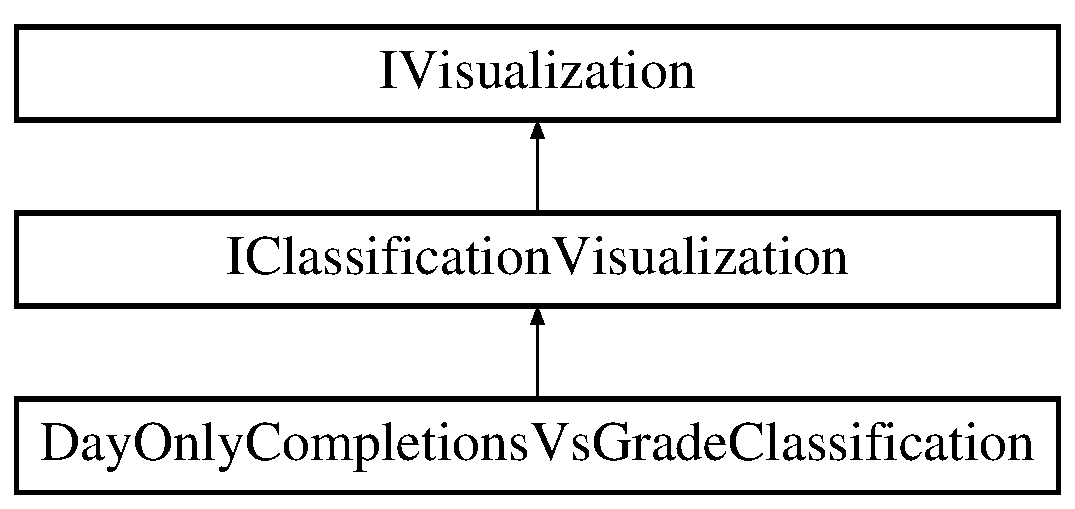
\includegraphics[height=3.000000cm]{classDayOnlyCompletionsVsGradeClassification}
\end{center}
\end{figure}
\subsection*{Public Member Functions}
\begin{DoxyCompactItemize}
\item 
\mbox{\Hypertarget{classDayOnlyCompletionsVsGradeClassification_a395e1c9dd3e409acebb7d31bdeadbd14}\label{classDayOnlyCompletionsVsGradeClassification_a395e1c9dd3e409acebb7d31bdeadbd14}} 
{\bfseries Day\+Only\+Completions\+Vs\+Grade\+Classification} (std\+::shared\+\_\+ptr$<$ \hyperlink{classIClassifier}{I\+Classifier} $>$ cl, std\+::shared\+\_\+ptr$<$ \hyperlink{classIFilter}{I\+Filter} $>$ gf, std\+::shared\+\_\+ptr$<$ \hyperlink{classIFilter}{I\+Filter} $>$ af)
\end{DoxyCompactItemize}


The documentation for this class was generated from the following files\+:\begin{DoxyCompactItemize}
\item 
Data\+Processer/src/\+Statistical\+Analyzer/\+Visualizations/Day\+Only\+Completions\+Vs\+Grade\+Classification.\+h\item 
Data\+Processer/src/\+Statistical\+Analyzer/\+Visualizations/Day\+Only\+Completions\+Vs\+Grade\+Classification.\+cpp\end{DoxyCompactItemize}

\hypertarget{classDayOnlyFilter}{}\section{Day\+Only\+Filter Class Reference}
\label{classDayOnlyFilter}\index{Day\+Only\+Filter@{Day\+Only\+Filter}}
Inheritance diagram for Day\+Only\+Filter\+:\begin{figure}[H]
\begin{center}
\leavevmode
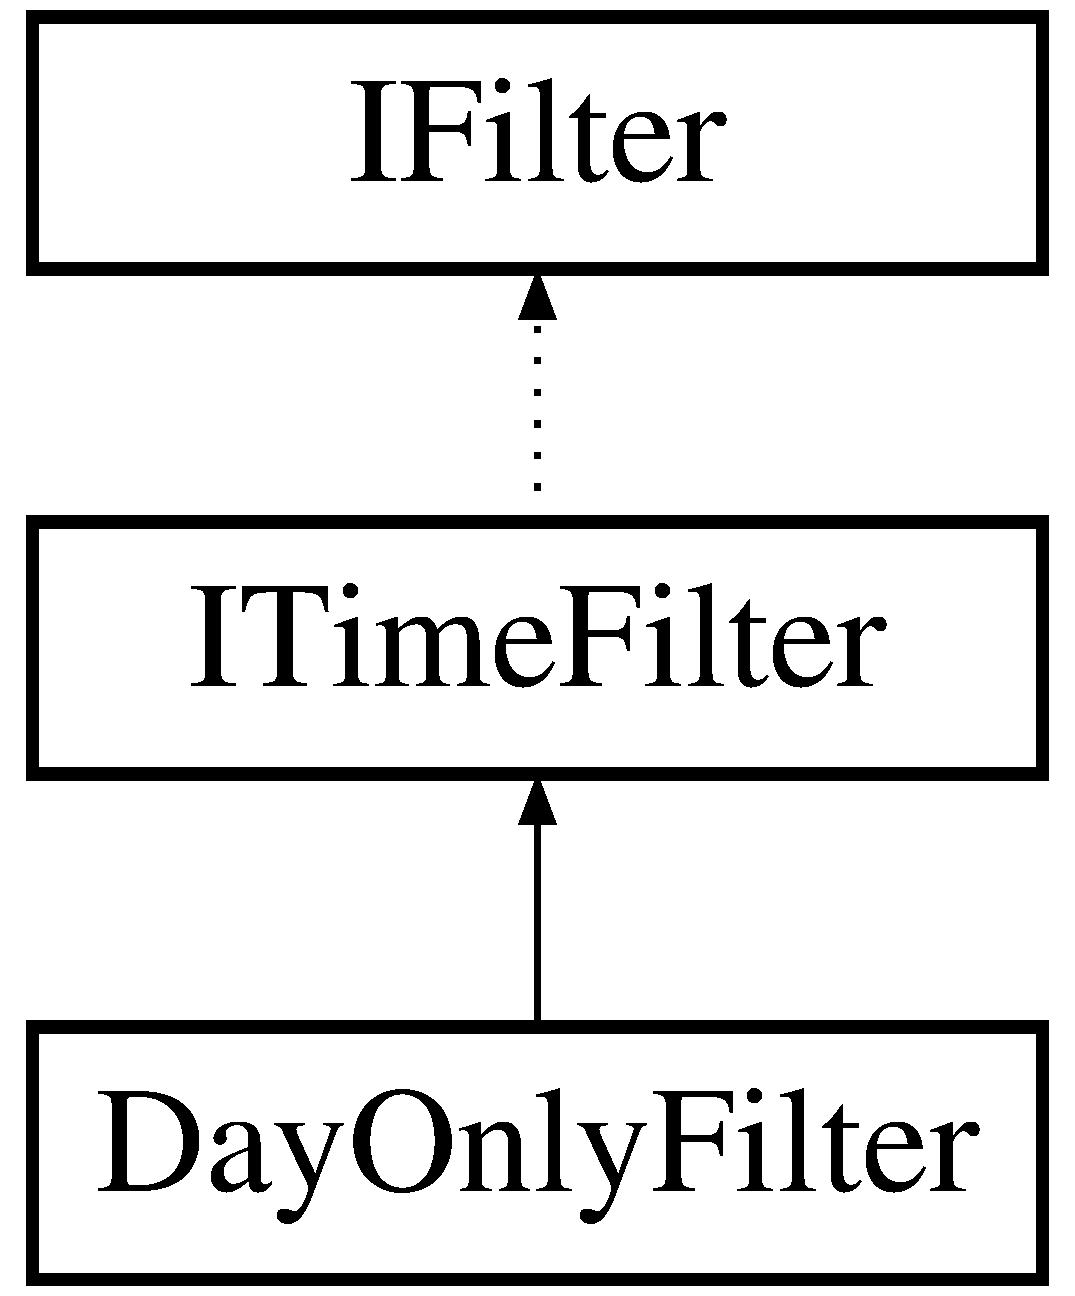
\includegraphics[height=3.000000cm]{classDayOnlyFilter}
\end{center}
\end{figure}
\subsection*{Public Member Functions}
\begin{DoxyCompactItemize}
\item 
\mbox{\Hypertarget{classDayOnlyFilter_a1f8472770c834980d9d6bf1e5095a7d4}\label{classDayOnlyFilter_a1f8472770c834980d9d6bf1e5095a7d4}} 
void {\bfseries set\+Filter\+Query\+Column\+Indexes} (\hyperlink{structFilterQueryColumnIndexes}{Filter\+Query\+Column\+Indexes} fq)
\item 
\mbox{\Hypertarget{classDayOnlyFilter_ad0a9e2504b6bdcb383c625c7c277c279}\label{classDayOnlyFilter_ad0a9e2504b6bdcb383c625c7c277c279}} 
\hyperlink{structFilterQueryColumnIndexes}{Filter\+Query\+Column\+Indexes} {\bfseries get\+Filter\+Query\+Column\+Indexes} ()
\end{DoxyCompactItemize}
\subsection*{Public Attributes}
\begin{DoxyCompactItemize}
\item 
\mbox{\Hypertarget{classDayOnlyFilter_aec030669d2438617efa3c7a68a199273}\label{classDayOnlyFilter_aec030669d2438617efa3c7a68a199273}} 
\hyperlink{structFilterQueryColumnIndexes}{Filter\+Query\+Column\+Indexes} {\bfseries query\+Column\+Indexes}
\end{DoxyCompactItemize}


The documentation for this class was generated from the following files\+:\begin{DoxyCompactItemize}
\item 
Data\+Processer/src/\+Statistical\+Analyzer/\+Filter/Day\+Only\+Filter.\+h\item 
Data\+Processer/src/\+Statistical\+Analyzer/\+Filter/Day\+Only\+Filter.\+cpp\end{DoxyCompactItemize}

\hypertarget{classDBSCAN}{}\section{D\+B\+S\+C\+AN Class Reference}
\label{classDBSCAN}\index{D\+B\+S\+C\+AN@{D\+B\+S\+C\+AN}}
\subsection*{Public Member Functions}
\begin{DoxyCompactItemize}
\item 
\mbox{\Hypertarget{classDBSCAN_addd367e6b66f8695d3e49817ae1210f7}\label{classDBSCAN_addd367e6b66f8695d3e49817ae1210f7}} 
std\+::vector$<$ std\+::vector$<$ std\+::shared\+\_\+ptr$<$ \hyperlink{classIClusteringPoint}{I\+Clustering\+Point} $>$ $>$ $>$ {\bfseries get\+Clustered\+Data} ()
\item 
\mbox{\Hypertarget{classDBSCAN_aaaf6f99736a6fbe4465dd2475f42d142}\label{classDBSCAN_aaaf6f99736a6fbe4465dd2475f42d142}} 
{\bfseries D\+B\+S\+C\+AN} (std\+::vector$<$ std\+::shared\+\_\+ptr$<$ \hyperlink{classDBScanPoint}{D\+B\+Scan\+Point} $>$$>$ p, int minpts, float maxradius)
\end{DoxyCompactItemize}


The documentation for this class was generated from the following files\+:\begin{DoxyCompactItemize}
\item 
Data\+Processer/src/\+Statistical\+Analyzer/\+D\+B\+S\+C\+A\+N/D\+B\+S\+C\+A\+N.\+h\item 
Data\+Processer/src/\+Statistical\+Analyzer/\+D\+B\+S\+C\+A\+N/D\+B\+S\+C\+A\+N.\+cpp\end{DoxyCompactItemize}

\hypertarget{classDBScanPoint}{}\section{D\+B\+Scan\+Point Class Reference}
\label{classDBScanPoint}\index{D\+B\+Scan\+Point@{D\+B\+Scan\+Point}}
Inheritance diagram for D\+B\+Scan\+Point\+:\begin{figure}[H]
\begin{center}
\leavevmode
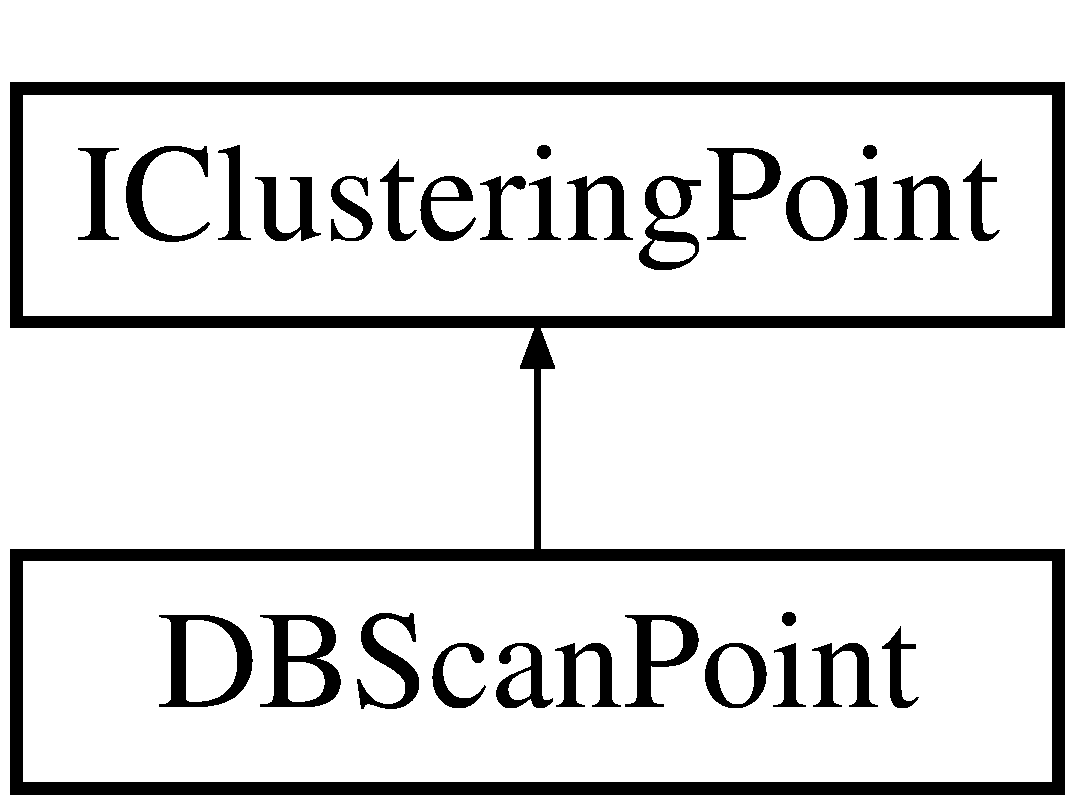
\includegraphics[height=2.000000cm]{classDBScanPoint}
\end{center}
\end{figure}
\subsection*{Public Member Functions}
\begin{DoxyCompactItemize}
\item 
\mbox{\Hypertarget{classDBScanPoint_a32cb3324ab1ad8c04916fc6ad8f6a47c}\label{classDBScanPoint_a32cb3324ab1ad8c04916fc6ad8f6a47c}} 
\hyperlink{classGenericVector}{Generic\+Vector} {\bfseries get\+Vector} () const
\item 
\mbox{\Hypertarget{classDBScanPoint_a66abde6747ff669c28e4091b771321d8}\label{classDBScanPoint_a66abde6747ff669c28e4091b771321d8}} 
int {\bfseries get\+Cluster\+Id} () const
\item 
\mbox{\Hypertarget{classDBScanPoint_abf0087ee6f609477ec784da2c0f9bc58}\label{classDBScanPoint_abf0087ee6f609477ec784da2c0f9bc58}} 
void {\bfseries set\+Vector} (\hyperlink{classGenericVector}{Generic\+Vector} new\+Vector)
\item 
\mbox{\Hypertarget{classDBScanPoint_a2c1b203f4f89ec227e5cc79d5ab8a3ea}\label{classDBScanPoint_a2c1b203f4f89ec227e5cc79d5ab8a3ea}} 
void {\bfseries set\+Cluster\+Id} (int new\+Cluster\+Id)
\item 
\mbox{\Hypertarget{classDBScanPoint_ae069327829be71239e11531b8ac76c93}\label{classDBScanPoint_ae069327829be71239e11531b8ac76c93}} 
{\bfseries D\+B\+Scan\+Point} (int c\+Id, \hyperlink{classGenericVector}{Generic\+Vector} v)
\end{DoxyCompactItemize}
\subsection*{Public Attributes}
\begin{DoxyCompactItemize}
\item 
\mbox{\Hypertarget{classDBScanPoint_a461918457f165af35a5ba75b9bec7276}\label{classDBScanPoint_a461918457f165af35a5ba75b9bec7276}} 
bool {\bfseries visited} = false
\item 
\mbox{\Hypertarget{classDBScanPoint_a3c7217821ce6d036cfb54a26b6e2bf0c}\label{classDBScanPoint_a3c7217821ce6d036cfb54a26b6e2bf0c}} 
bool {\bfseries is\+Noise} = false
\item 
\mbox{\Hypertarget{classDBScanPoint_a474f0b933ad12fa225c780498b66f2c4}\label{classDBScanPoint_a474f0b933ad12fa225c780498b66f2c4}} 
\hyperlink{classGenericVector}{Generic\+Vector} {\bfseries vector}
\item 
\mbox{\Hypertarget{classDBScanPoint_aa791e2035bf72a15e02eaa81b7fe2a4c}\label{classDBScanPoint_aa791e2035bf72a15e02eaa81b7fe2a4c}} 
int {\bfseries cluster\+Id}
\end{DoxyCompactItemize}


The documentation for this class was generated from the following file\+:\begin{DoxyCompactItemize}
\item 
Data\+Processer/src/\+Statistical\+Analyzer/\+Point/D\+B\+Scan\+Point.\+h\end{DoxyCompactItemize}

\hypertarget{classExcersiseCompletionAndGradesClustering}{}\section{Excersise\+Completion\+And\+Grades\+Clustering Class Reference}
\label{classExcersiseCompletionAndGradesClustering}\index{Excersise\+Completion\+And\+Grades\+Clustering@{Excersise\+Completion\+And\+Grades\+Clustering}}
Inheritance diagram for Excersise\+Completion\+And\+Grades\+Clustering\+:\begin{figure}[H]
\begin{center}
\leavevmode
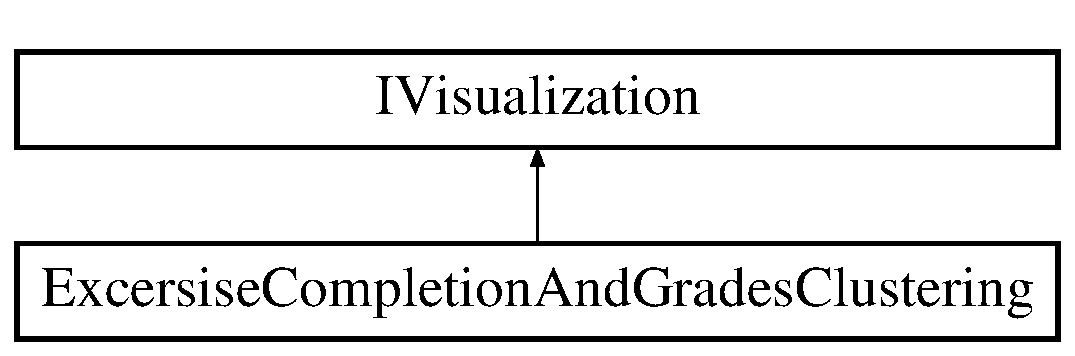
\includegraphics[height=2.000000cm]{classExcersiseCompletionAndGradesClustering}
\end{center}
\end{figure}
\subsection*{Public Member Functions}
\begin{DoxyCompactItemize}
\item 
\mbox{\Hypertarget{classExcersiseCompletionAndGradesClustering_ac1dd40e96f2b6ecee0c51d6e9ba5da45}\label{classExcersiseCompletionAndGradesClustering_ac1dd40e96f2b6ecee0c51d6e9ba5da45}} 
virtual std\+::string {\bfseries get\+Visualization\+As\+J\+S\+ON} ()
\item 
\mbox{\Hypertarget{classExcersiseCompletionAndGradesClustering_a4ca7007ff3558749c5922bfa57b97ab7}\label{classExcersiseCompletionAndGradesClustering_a4ca7007ff3558749c5922bfa57b97ab7}} 
std\+::vector$<$ std\+::vector$<$ std\+::shared\+\_\+ptr$<$ \hyperlink{classIClusteringPoint}{I\+Clustering\+Point} $>$ $>$ $>$ {\bfseries get\+Excersise\+Completion\+And\+Grades\+Clusters} ()
\item 
\mbox{\Hypertarget{classExcersiseCompletionAndGradesClustering_a8c2b6e42157a4c4e660daa4b837da126}\label{classExcersiseCompletionAndGradesClustering_a8c2b6e42157a4c4e660daa4b837da126}} 
std\+::map$<$ std\+::string, std\+::pair$<$ int, int $>$ $>$ {\bfseries get\+Amount\+Of\+Exercises\+Completed\+And\+Grades\+Per\+Student} ()
\item 
\mbox{\Hypertarget{classExcersiseCompletionAndGradesClustering_a8fed3c9cfe2dcffa141db566947dafa9}\label{classExcersiseCompletionAndGradesClustering_a8fed3c9cfe2dcffa141db566947dafa9}} 
{\bfseries Excersise\+Completion\+And\+Grades\+Clustering} (std\+::shared\+\_\+ptr$<$ \hyperlink{classIFilter}{I\+Filter} $>$ gf, std\+::shared\+\_\+ptr$<$ \hyperlink{classIFilter}{I\+Filter} $>$ af, std\+::shared\+\_\+ptr$<$ \hyperlink{classITimeFilter}{I\+Time\+Filter} $>$ df)
\end{DoxyCompactItemize}


The documentation for this class was generated from the following files\+:\begin{DoxyCompactItemize}
\item 
Data\+Processer/src/\+Statistical\+Analyzer/\+Visualizations/Excersise\+Completion\+And\+Grades\+Clustering.\+h\item 
Data\+Processer/src/\+Statistical\+Analyzer/\+Visualizations/Excersise\+Completion\+And\+Grades\+Clustering.\+cpp\end{DoxyCompactItemize}

\hypertarget{structFilterContext}{}\section{Filter\+Context Struct Reference}
\label{structFilterContext}\index{Filter\+Context@{Filter\+Context}}
\subsection*{Public Attributes}
\begin{DoxyCompactItemize}
\item 
\mbox{\Hypertarget{structFilterContext_a5028f286271d4ff440b30eb2ad7f4b66}\label{structFilterContext_a5028f286271d4ff440b30eb2ad7f4b66}} 
double {\bfseries time\+Between\+Assignments\+Threshold} = 1
\item 
\mbox{\Hypertarget{structFilterContext_a322a08000ce440bd2df4f1623d514877}\label{structFilterContext_a322a08000ce440bd2df4f1623d514877}} 
double {\bfseries upper\+Percentage\+Of\+Grades\+To\+Be\+Selected} = 100
\end{DoxyCompactItemize}


The documentation for this struct was generated from the following file\+:\begin{DoxyCompactItemize}
\item 
Data\+Processer/src/\+Statistical\+Analyzer/\+Filter/I\+Filter.\+h\end{DoxyCompactItemize}

\hypertarget{structFilterQueryColumnIndexes}{}\section{Filter\+Query\+Column\+Indexes Struct Reference}
\label{structFilterQueryColumnIndexes}\index{Filter\+Query\+Column\+Indexes@{Filter\+Query\+Column\+Indexes}}
\subsection*{Public Attributes}
\begin{DoxyCompactItemize}
\item 
\mbox{\Hypertarget{structFilterQueryColumnIndexes_ae2be76e71ebf2718ad78161781ed7e44}\label{structFilterQueryColumnIndexes_ae2be76e71ebf2718ad78161781ed7e44}} 
int {\bfseries student\+Id\+Column\+Index}
\item 
\mbox{\Hypertarget{structFilterQueryColumnIndexes_a3db0840c5f0343b63bd08d6444ac0f3e}\label{structFilterQueryColumnIndexes_a3db0840c5f0343b63bd08d6444ac0f3e}} 
int {\bfseries timestamp\+Index}
\end{DoxyCompactItemize}


The documentation for this struct was generated from the following file\+:\begin{DoxyCompactItemize}
\item 
Data\+Processer/src/\+Statistical\+Analyzer/\+Filter/I\+Filter.\+h\end{DoxyCompactItemize}

\hypertarget{classGenericVector}{}\section{Generic\+Vector Class Reference}
\label{classGenericVector}\index{Generic\+Vector@{Generic\+Vector}}
\subsection*{Public Member Functions}
\begin{DoxyCompactItemize}
\item 
\mbox{\Hypertarget{classGenericVector_a95df0a51a505c9b6b864993d1979b95b}\label{classGenericVector_a95df0a51a505c9b6b864993d1979b95b}} 
{\bfseries Generic\+Vector} (pair$<$ float, float $>$ p)
\item 
\mbox{\Hypertarget{classGenericVector_abf78215cf06a38dd61c627684a45524b}\label{classGenericVector_abf78215cf06a38dd61c627684a45524b}} 
{\bfseries Generic\+Vector} (vector$<$ float $>$ v)
\item 
\mbox{\Hypertarget{classGenericVector_a994ddf14b55ac6e9333d676cbb9a5278}\label{classGenericVector_a994ddf14b55ac6e9333d676cbb9a5278}} 
float {\bfseries dot\+Product} (\hyperlink{classGenericVector}{Generic\+Vector} \&other)
\item 
\mbox{\Hypertarget{classGenericVector_a26331bc15f84f065b762b19d9e725106}\label{classGenericVector_a26331bc15f84f065b762b19d9e725106}} 
float {\bfseries get\+Euclid\+Distance} (\hyperlink{classGenericVector}{Generic\+Vector} \&other)
\item 
\mbox{\Hypertarget{classGenericVector_acf8ce1f677921e004ab98abca13d60e9}\label{classGenericVector_acf8ce1f677921e004ab98abca13d60e9}} 
void {\bfseries sum\+With} (\hyperlink{classGenericVector}{Generic\+Vector} \&gv2)
\item 
\mbox{\Hypertarget{classGenericVector_af6f9eafb78d6ad371aa3397dac484c2e}\label{classGenericVector_af6f9eafb78d6ad371aa3397dac484c2e}} 
\hyperlink{classGenericVector}{Generic\+Vector} {\bfseries divide} (int divisor)
\item 
\mbox{\Hypertarget{classGenericVector_a21c1f751fc162ea0bf6bccfad7fa4afa}\label{classGenericVector_a21c1f751fc162ea0bf6bccfad7fa4afa}} 
bool {\bfseries is\+Not\+Equal} (\hyperlink{classGenericVector}{Generic\+Vector} \&other)
\item 
\mbox{\Hypertarget{classGenericVector_a38a8455e8c908b9a0026087a8a5f66ac}\label{classGenericVector_a38a8455e8c908b9a0026087a8a5f66ac}} 
bool {\bfseries Vector\+Sizes\+Equal} (\hyperlink{classGenericVector}{Generic\+Vector} \&other)
\item 
\mbox{\Hypertarget{classGenericVector_a20588c7f40fe6a53899c952dd3dc2285}\label{classGenericVector_a20588c7f40fe6a53899c952dd3dc2285}} 
string {\bfseries To\+String} ()
\end{DoxyCompactItemize}
\subsection*{Static Public Member Functions}
\begin{DoxyCompactItemize}
\item 
\mbox{\Hypertarget{classGenericVector_a164eb902cb77e118826a335edbbf3f35}\label{classGenericVector_a164eb902cb77e118826a335edbbf3f35}} 
static \hyperlink{classGenericVector}{Generic\+Vector} {\bfseries get\+Random\+Vector} (int dimension\+Length)
\end{DoxyCompactItemize}
\subsection*{Public Attributes}
\begin{DoxyCompactItemize}
\item 
\mbox{\Hypertarget{classGenericVector_a80fb20717e0826df7fd71f84491bc648}\label{classGenericVector_a80fb20717e0826df7fd71f84491bc648}} 
vector$<$ float $>$ {\bfseries values}
\end{DoxyCompactItemize}


The documentation for this class was generated from the following files\+:\begin{DoxyCompactItemize}
\item 
Data\+Processer/src/\+Statistical\+Analyzer/\+Generic\+Vector/Generic\+Vector.\+h\item 
Data\+Processer/src/\+Statistical\+Analyzer/\+Generic\+Vector/Generic\+Vector.\+cpp\end{DoxyCompactItemize}

\hypertarget{classGradeAndExcersiseSuccesses}{}\section{Grade\+And\+Excersise\+Successes Class Reference}
\label{classGradeAndExcersiseSuccesses}\index{Grade\+And\+Excersise\+Successes@{Grade\+And\+Excersise\+Successes}}
Inheritance diagram for Grade\+And\+Excersise\+Successes\+:\begin{figure}[H]
\begin{center}
\leavevmode
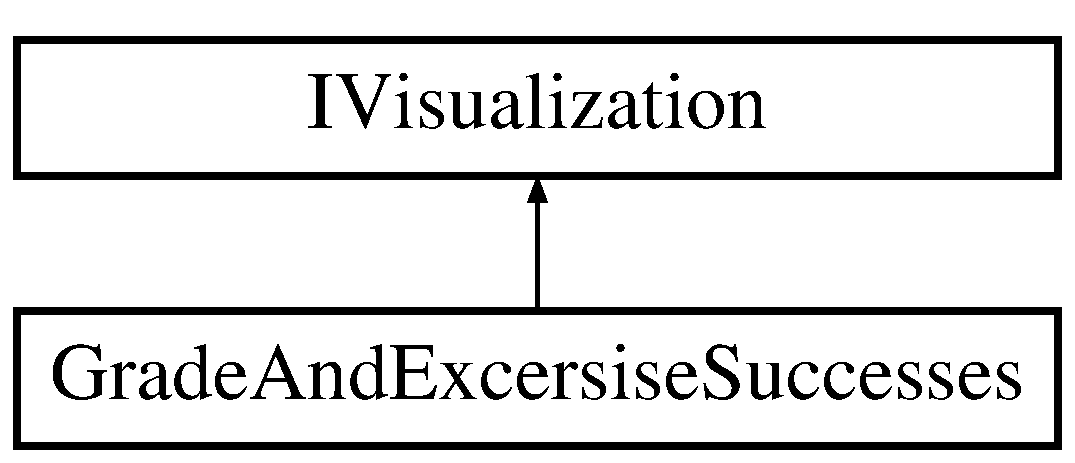
\includegraphics[height=2.000000cm]{classGradeAndExcersiseSuccesses}
\end{center}
\end{figure}
\subsection*{Public Member Functions}
\begin{DoxyCompactItemize}
\item 
\mbox{\Hypertarget{classGradeAndExcersiseSuccesses_a98ca9e2045f7d15e9a90a03fb7ea30ce}\label{classGradeAndExcersiseSuccesses_a98ca9e2045f7d15e9a90a03fb7ea30ce}} 
std\+::string {\bfseries get\+Visualization\+As\+J\+S\+ON} ()
\item 
\mbox{\Hypertarget{classGradeAndExcersiseSuccesses_a0d735be765216f11a24d829c383373f8}\label{classGradeAndExcersiseSuccesses_a0d735be765216f11a24d829c383373f8}} 
{\bfseries Grade\+And\+Excersise\+Successes} (std\+::shared\+\_\+ptr$<$ \hyperlink{classIFilter}{I\+Filter} $>$ gf, std\+::shared\+\_\+ptr$<$ \hyperlink{classIFilter}{I\+Filter} $>$ af, std\+::shared\+\_\+ptr$<$ \hyperlink{classITimeFilter}{I\+Time\+Filter} $>$ df)
\end{DoxyCompactItemize}


The documentation for this class was generated from the following files\+:\begin{DoxyCompactItemize}
\item 
Data\+Processer/src/\+Statistical\+Analyzer/\+Visualizations/Grade\+And\+Excersise\+Successes.\+h\item 
Data\+Processer/src/\+Statistical\+Analyzer/\+Visualizations/Grade\+And\+Excersise\+Successes.\+cpp\end{DoxyCompactItemize}

\hypertarget{classGradeAvgsPerClass}{}\section{Grade\+Avgs\+Per\+Class Class Reference}
\label{classGradeAvgsPerClass}\index{Grade\+Avgs\+Per\+Class@{Grade\+Avgs\+Per\+Class}}
Inheritance diagram for Grade\+Avgs\+Per\+Class\+:\begin{figure}[H]
\begin{center}
\leavevmode
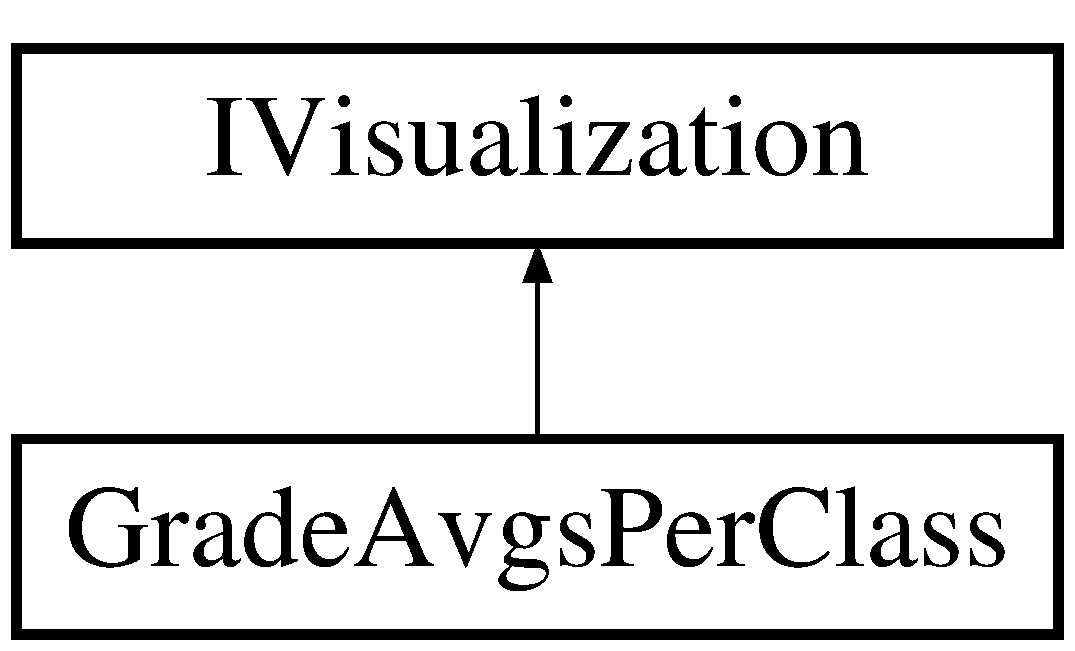
\includegraphics[height=2.000000cm]{classGradeAvgsPerClass}
\end{center}
\end{figure}
\subsection*{Public Member Functions}
\begin{DoxyCompactItemize}
\item 
\mbox{\Hypertarget{classGradeAvgsPerClass_ab87b0c0c7365150ff345cbf49af916da}\label{classGradeAvgsPerClass_ab87b0c0c7365150ff345cbf49af916da}} 
std\+::string {\bfseries get\+Visualization\+As\+J\+S\+ON} ()
\end{DoxyCompactItemize}


The documentation for this class was generated from the following files\+:\begin{DoxyCompactItemize}
\item 
Data\+Processer/src/\+Statistical\+Analyzer/\+Visualizations/Grade\+Avgs\+Per\+Class.\+h\item 
Data\+Processer/src/\+Statistical\+Analyzer/\+Visualizations/Grade\+Avgs\+Per\+Class.\+cpp\end{DoxyCompactItemize}

\hypertarget{classGradePercentageFilter}{}\section{Grade\+Percentage\+Filter Class Reference}
\label{classGradePercentageFilter}\index{Grade\+Percentage\+Filter@{Grade\+Percentage\+Filter}}
Inheritance diagram for Grade\+Percentage\+Filter\+:\begin{figure}[H]
\begin{center}
\leavevmode
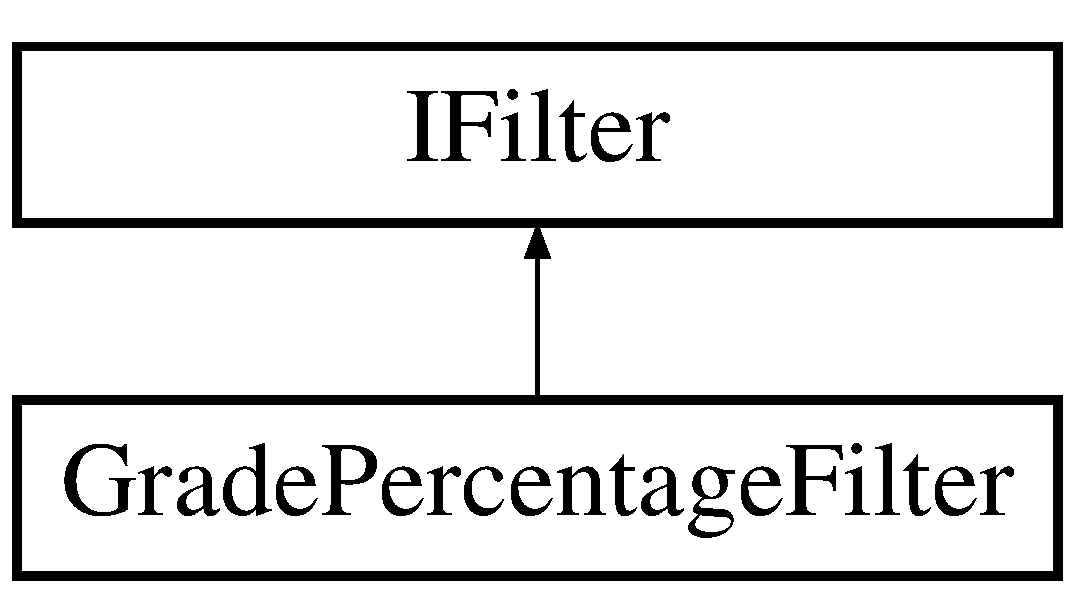
\includegraphics[height=2.000000cm]{classGradePercentageFilter}
\end{center}
\end{figure}
\subsection*{Public Member Functions}
\begin{DoxyCompactItemize}
\item 
\mbox{\Hypertarget{classGradePercentageFilter_ac7a84e4ac69a5a8b34dab99a607bd2c6}\label{classGradePercentageFilter_ac7a84e4ac69a5a8b34dab99a607bd2c6}} 
void {\bfseries set\+Filter\+Query\+Column\+Indexes} (\hyperlink{structFilterQueryColumnIndexes}{Filter\+Query\+Column\+Indexes} fq)
\item 
\mbox{\Hypertarget{classGradePercentageFilter_a742c141c49cfdfbbaa24bf591e7e5372}\label{classGradePercentageFilter_a742c141c49cfdfbbaa24bf591e7e5372}} 
\hyperlink{structFilterQueryColumnIndexes}{Filter\+Query\+Column\+Indexes} {\bfseries get\+Filter\+Query\+Column\+Indexes} ()
\item 
\mbox{\Hypertarget{classGradePercentageFilter_a2037adfc91055fdf4f325bfe9e32c679}\label{classGradePercentageFilter_a2037adfc91055fdf4f325bfe9e32c679}} 
void {\bfseries set\+Filter\+Context} (\hyperlink{structFilterContext}{Filter\+Context} fc)
\item 
\mbox{\Hypertarget{classGradePercentageFilter_ad21749352c3b56e1675535e008ff5c00}\label{classGradePercentageFilter_ad21749352c3b56e1675535e008ff5c00}} 
\hyperlink{structFilterContext}{Filter\+Context} {\bfseries get\+Filter\+Context} ()
\item 
\mbox{\Hypertarget{classGradePercentageFilter_ab89b43a19f6bdc7f15421cd4b8747ad2}\label{classGradePercentageFilter_ab89b43a19f6bdc7f15421cd4b8747ad2}} 
std\+::vector$<$ pqxx\+::result\+::tuple $>$ {\bfseries filter} (vector$<$ pqxx\+::result\+::tuple $>$ unfiltered\+Rows)
\item 
\mbox{\Hypertarget{classGradePercentageFilter_adc5a15db768c64778c59ff651b19aa29}\label{classGradePercentageFilter_adc5a15db768c64778c59ff651b19aa29}} 
{\bfseries Grade\+Percentage\+Filter} (\hyperlink{structFilterContext}{Filter\+Context} f)
\end{DoxyCompactItemize}
\subsection*{Public Attributes}
\begin{DoxyCompactItemize}
\item 
\mbox{\Hypertarget{classGradePercentageFilter_a9d910bae10fff054b968853e34a83d79}\label{classGradePercentageFilter_a9d910bae10fff054b968853e34a83d79}} 
\hyperlink{structFilterQueryColumnIndexes}{Filter\+Query\+Column\+Indexes} {\bfseries query\+Column\+Indexes}
\item 
\mbox{\Hypertarget{classGradePercentageFilter_afd8e2a3bca8b2ca675f52ed5dd9c4e37}\label{classGradePercentageFilter_afd8e2a3bca8b2ca675f52ed5dd9c4e37}} 
\hyperlink{structFilterContext}{Filter\+Context} {\bfseries filter\+Context}
\end{DoxyCompactItemize}


The documentation for this class was generated from the following files\+:\begin{DoxyCompactItemize}
\item 
Data\+Processer/src/\+Statistical\+Analyzer/\+Filter/Grade\+Percentage\+Filter.\+h\item 
Data\+Processer/src/\+Statistical\+Analyzer/\+Filter/Grade\+Percentage\+Filter.\+cpp\end{DoxyCompactItemize}

\hypertarget{classIClassificationVisualization}{}\section{I\+Classification\+Visualization Class Reference}
\label{classIClassificationVisualization}\index{I\+Classification\+Visualization@{I\+Classification\+Visualization}}
Inheritance diagram for I\+Classification\+Visualization\+:\begin{figure}[H]
\begin{center}
\leavevmode
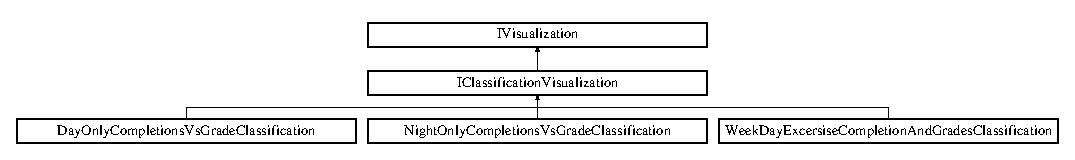
\includegraphics[height=1.696970cm]{classIClassificationVisualization}
\end{center}
\end{figure}
\subsection*{Public Member Functions}
\begin{DoxyCompactItemize}
\item 
\mbox{\Hypertarget{classIClassificationVisualization_a0ccbaa688c997957f8027a0ea74bcc6f}\label{classIClassificationVisualization_a0ccbaa688c997957f8027a0ea74bcc6f}} 
virtual std\+::string {\bfseries get\+Visualization\+As\+J\+S\+ON} ()
\end{DoxyCompactItemize}


The documentation for this class was generated from the following file\+:\begin{DoxyCompactItemize}
\item 
Data\+Processer/src/\+Statistical\+Analyzer/\+Visualizations/I\+Classification\+Visualization.\+h\end{DoxyCompactItemize}

\hypertarget{classIClassifier}{}\section{I\+Classifier Class Reference}
\label{classIClassifier}\index{I\+Classifier@{I\+Classifier}}


{\ttfamily \#include $<$I\+Classifier.\+h$>$}

Inheritance diagram for I\+Classifier\+:\begin{figure}[H]
\begin{center}
\leavevmode
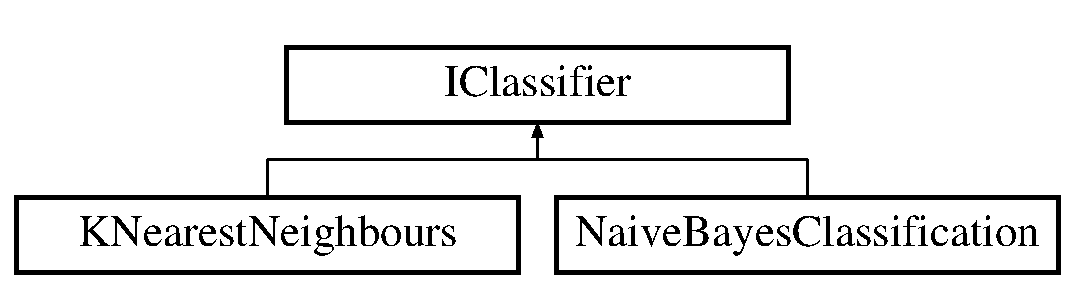
\includegraphics[height=2.000000cm]{classIClassifier}
\end{center}
\end{figure}
\subsection*{Public Member Functions}
\begin{DoxyCompactItemize}
\item 
\mbox{\Hypertarget{classIClassifier_ae16ef894fd72f4d94986f6d68a9d43c5}\label{classIClassifier_ae16ef894fd72f4d94986f6d68a9d43c5}} 
virtual std\+::vector$<$ std\+::vector$<$ std\+::shared\+\_\+ptr$<$ \hyperlink{classIClusteringPoint}{I\+Clustering\+Point} $>$ $>$ $>$ {\bfseries get\+Classified\+Points} ()=0
\item 
\mbox{\Hypertarget{classIClassifier_ab0033ae8e780d741ff1d70c4473ee385}\label{classIClassifier_ab0033ae8e780d741ff1d70c4473ee385}} 
virtual void {\bfseries initialize} (std\+::vector$<$ std\+::shared\+\_\+ptr$<$ \hyperlink{classIClusteringPoint}{I\+Clustering\+Point} $>$$>$ input, vector$<$ vector$<$ std\+::shared\+\_\+ptr$<$ \hyperlink{classIClusteringPoint}{I\+Clustering\+Point} $>$$>$$>$ tc)=0
\end{DoxyCompactItemize}


\subsection{Detailed Description}
Each derived class \hyperlink{classIClassifier}{I\+Classifier} overrides the virtual \textquotesingle{}get\+Classified\+Points\textquotesingle{} and \textquotesingle{}initialize\textquotesingle{} methods. \textquotesingle{}initialize\textquotesingle{} simulates a virtual constructor (which does not exist in C++) 

The documentation for this class was generated from the following file\+:\begin{DoxyCompactItemize}
\item 
Data\+Processer/src/\+Statistical\+Analyzer/\+Classifiers/I\+Classifier.\+h\end{DoxyCompactItemize}

\hypertarget{classIClusteringPoint}{}\section{I\+Clustering\+Point Class Reference}
\label{classIClusteringPoint}\index{I\+Clustering\+Point@{I\+Clustering\+Point}}
Inheritance diagram for I\+Clustering\+Point\+:\begin{figure}[H]
\begin{center}
\leavevmode
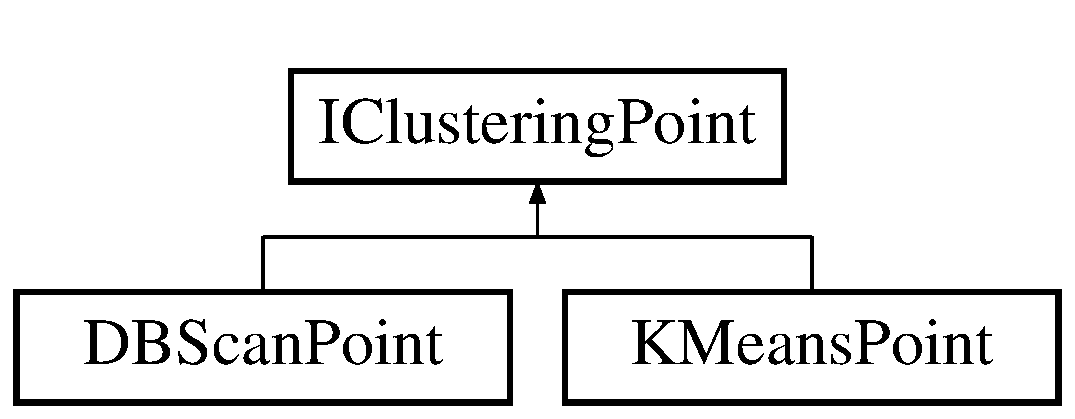
\includegraphics[height=2.000000cm]{classIClusteringPoint}
\end{center}
\end{figure}
\subsection*{Public Member Functions}
\begin{DoxyCompactItemize}
\item 
\mbox{\Hypertarget{classIClusteringPoint_a809b5184b30f8fac488345805867fbb2}\label{classIClusteringPoint_a809b5184b30f8fac488345805867fbb2}} 
virtual \hyperlink{classGenericVector}{Generic\+Vector} {\bfseries get\+Vector} () const =0
\item 
\mbox{\Hypertarget{classIClusteringPoint_a51707c3f5009bac076a2869237e1b3c1}\label{classIClusteringPoint_a51707c3f5009bac076a2869237e1b3c1}} 
virtual int {\bfseries get\+Cluster\+Id} () const =0
\item 
\mbox{\Hypertarget{classIClusteringPoint_a9f8f45aa838b3d416cd4130bee795bbd}\label{classIClusteringPoint_a9f8f45aa838b3d416cd4130bee795bbd}} 
virtual void {\bfseries set\+Vector} (\hyperlink{classGenericVector}{Generic\+Vector} new\+Vector)=0
\item 
\mbox{\Hypertarget{classIClusteringPoint_a0f6f914435a436a798d64ac7d118629a}\label{classIClusteringPoint_a0f6f914435a436a798d64ac7d118629a}} 
virtual void {\bfseries set\+Cluster\+Id} (int new\+Centroid\+Id)=0
\item 
\mbox{\Hypertarget{classIClusteringPoint_a42bcbacc21a04dc705657e1e21c15d84}\label{classIClusteringPoint_a42bcbacc21a04dc705657e1e21c15d84}} 
bool {\bfseries operator$<$} (const \hyperlink{classIClusteringPoint}{I\+Clustering\+Point} \&other) const
\item 
\mbox{\Hypertarget{classIClusteringPoint_aafcde65042318fee89f7e45b0d66ec70}\label{classIClusteringPoint_aafcde65042318fee89f7e45b0d66ec70}} 
bool {\bfseries operator==} (const \hyperlink{classIClusteringPoint}{I\+Clustering\+Point} \&other) const
\end{DoxyCompactItemize}


The documentation for this class was generated from the following file\+:\begin{DoxyCompactItemize}
\item 
Data\+Processer/src/\+Statistical\+Analyzer/\+Point/I\+Clustering\+Point.\+h\end{DoxyCompactItemize}

\hypertarget{classIFilter}{}\section{I\+Filter Class Reference}
\label{classIFilter}\index{I\+Filter@{I\+Filter}}
Inheritance diagram for I\+Filter\+:\begin{figure}[H]
\begin{center}
\leavevmode
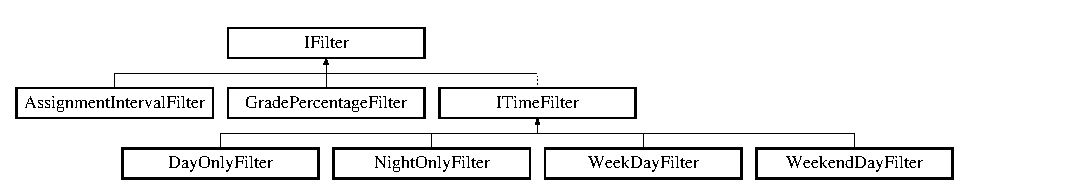
\includegraphics[height=2.167742cm]{classIFilter}
\end{center}
\end{figure}
\subsection*{Public Member Functions}
\begin{DoxyCompactItemize}
\item 
\mbox{\Hypertarget{classIFilter_ad66e2b3f6268436f2b7b127dab38633d}\label{classIFilter_ad66e2b3f6268436f2b7b127dab38633d}} 
virtual void {\bfseries set\+Filter\+Query\+Column\+Indexes} (\hyperlink{structFilterQueryColumnIndexes}{Filter\+Query\+Column\+Indexes} fq)
\item 
\mbox{\Hypertarget{classIFilter_aab274a76ddbba2591c9112edf4bfbc26}\label{classIFilter_aab274a76ddbba2591c9112edf4bfbc26}} 
virtual \hyperlink{structFilterQueryColumnIndexes}{Filter\+Query\+Column\+Indexes} {\bfseries get\+Filter\+Query\+Column\+Indexes} ()
\item 
\mbox{\Hypertarget{classIFilter_a1ab08052b3949763ea2f0dd04a05030b}\label{classIFilter_a1ab08052b3949763ea2f0dd04a05030b}} 
virtual void {\bfseries set\+Filter\+Context} (\hyperlink{structFilterContext}{Filter\+Context} fc)
\item 
\mbox{\Hypertarget{classIFilter_a5e3249740f7f913a03d09f4437d98be4}\label{classIFilter_a5e3249740f7f913a03d09f4437d98be4}} 
virtual \hyperlink{structFilterContext}{Filter\+Context} {\bfseries get\+Filter\+Context} ()
\item 
\mbox{\Hypertarget{classIFilter_a3abe23670a8b3641fae336cf5efdb775}\label{classIFilter_a3abe23670a8b3641fae336cf5efdb775}} 
virtual std\+::vector$<$ pqxx\+::result\+::tuple $>$ {\bfseries filter} (std\+::vector$<$ pqxx\+::result\+::tuple $>$ unfiltered\+Rows)=0
\end{DoxyCompactItemize}


The documentation for this class was generated from the following file\+:\begin{DoxyCompactItemize}
\item 
Data\+Processer/src/\+Statistical\+Analyzer/\+Filter/I\+Filter.\+h\end{DoxyCompactItemize}

\hypertarget{classIRegression}{}\section{I\+Regression Class Reference}
\label{classIRegression}\index{I\+Regression@{I\+Regression}}


{\ttfamily \#include $<$I\+Regression.\+h$>$}

Inheritance diagram for I\+Regression\+:\begin{figure}[H]
\begin{center}
\leavevmode
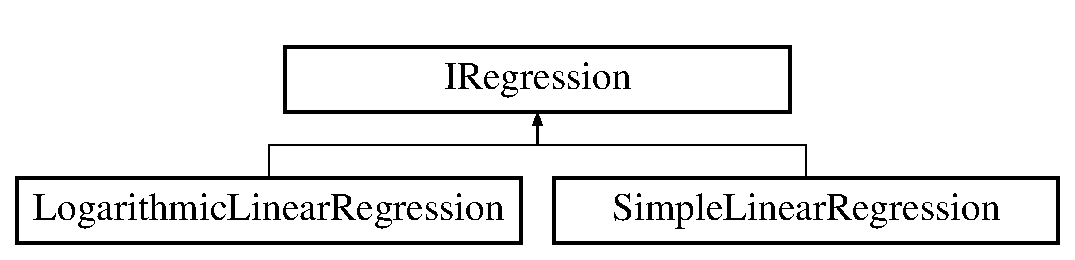
\includegraphics[height=2.000000cm]{classIRegression}
\end{center}
\end{figure}
\subsection*{Public Member Functions}
\begin{DoxyCompactItemize}
\item 
\mbox{\Hypertarget{classIRegression_ae8f41b89c9d8547d1d03749ac9ba9f4b}\label{classIRegression_ae8f41b89c9d8547d1d03749ac9ba9f4b}} 
virtual std\+::string {\bfseries get\+Regression\+As\+J\+S\+ON} ()=0
\item 
\mbox{\Hypertarget{classIRegression_a96ea1a25100c62c8fff0b6c8c134946c}\label{classIRegression_a96ea1a25100c62c8fff0b6c8c134946c}} 
{\bfseries I\+Regression} (std\+::vector$<$ std\+::pair$<$ float, float $>$$>$ p)
\end{DoxyCompactItemize}
\subsection*{Protected Member Functions}
\begin{DoxyCompactItemize}
\item 
\mbox{\Hypertarget{classIRegression_a98c5a0c7bc09079c42239f9b765a9c88}\label{classIRegression_a98c5a0c7bc09079c42239f9b765a9c88}} 
std\+::pair$<$ \hyperlink{classGenericVector}{Generic\+Vector}, \hyperlink{classGenericVector}{Generic\+Vector} $>$ {\bfseries convert\+Pairs\+To\+G\+Vs} (std\+::vector$<$ std\+::pair$<$ float, float $>$$>$ pairs)
\item 
\mbox{\Hypertarget{classIRegression_a8790d7641b1ade722715e5d8bf473344}\label{classIRegression_a8790d7641b1ade722715e5d8bf473344}} 
virtual float {\bfseries get\+Slope} ()=0
\item 
\mbox{\Hypertarget{classIRegression_a5a1a2500a739b98435563e5115576228}\label{classIRegression_a5a1a2500a739b98435563e5115576228}} 
virtual float {\bfseries get\+Intercept} ()=0
\item 
\mbox{\Hypertarget{classIRegression_af62863f66e768a0bb482000862b16164}\label{classIRegression_af62863f66e768a0bb482000862b16164}} 
virtual std\+::vector$<$ std\+::pair$<$ float, float $>$ $>$ {\bfseries get\+Regression} ()=0
\end{DoxyCompactItemize}
\subsection*{Protected Attributes}
\begin{DoxyCompactItemize}
\item 
\mbox{\Hypertarget{classIRegression_abdce3eb0c896fe60b6c272060eab7860}\label{classIRegression_abdce3eb0c896fe60b6c272060eab7860}} 
std\+::pair$<$ \hyperlink{classGenericVector}{Generic\+Vector}, \hyperlink{classGenericVector}{Generic\+Vector} $>$ {\bfseries x\+And\+Y\+Vectors}
\end{DoxyCompactItemize}


\subsection{Detailed Description}
Each \hyperlink{classIRegression}{I\+Regression} has to define its\textquotesingle{} own ways of calculating slope, intercept and final regression. \textquotesingle{}get\+Regression\+As\+J\+S\+ON\textquotesingle{} is specific per \hyperlink{classIRegression}{I\+Regression} derived class as well. 

The documentation for this class was generated from the following files\+:\begin{DoxyCompactItemize}
\item 
Data\+Processer/src/\+Statistical\+Analyzer/\+Regression/I\+Regression.\+h\item 
Data\+Processer/src/\+Statistical\+Analyzer/\+Regression/I\+Regression.\+cpp\end{DoxyCompactItemize}

\hypertarget{classITimeFilter}{}\section{I\+Time\+Filter Class Reference}
\label{classITimeFilter}\index{I\+Time\+Filter@{I\+Time\+Filter}}
Inheritance diagram for I\+Time\+Filter\+:\begin{figure}[H]
\begin{center}
\leavevmode
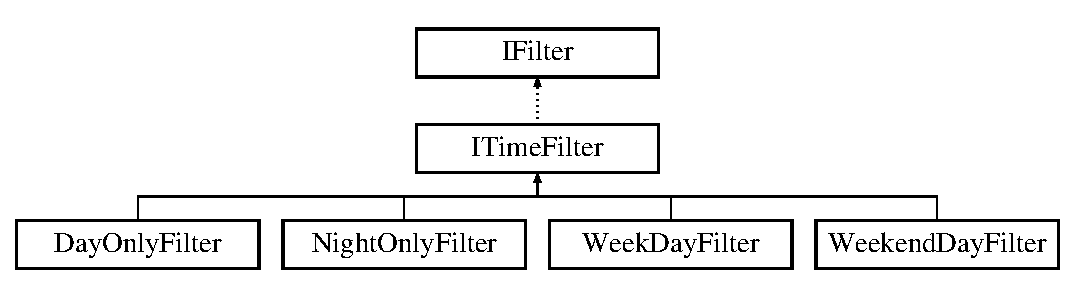
\includegraphics[height=3.000000cm]{classITimeFilter}
\end{center}
\end{figure}
\subsection*{Public Member Functions}
\begin{DoxyCompactItemize}
\item 
\mbox{\Hypertarget{classITimeFilter_ab4eaa567bbbc24f5ad60d098cb1e8f42}\label{classITimeFilter_ab4eaa567bbbc24f5ad60d098cb1e8f42}} 
void {\bfseries set\+Filter\+Query\+Column\+Indexes} (\hyperlink{structFilterQueryColumnIndexes}{Filter\+Query\+Column\+Indexes} fq)
\item 
\mbox{\Hypertarget{classITimeFilter_a5f9b872405149c0ae2f02b0e25501ea3}\label{classITimeFilter_a5f9b872405149c0ae2f02b0e25501ea3}} 
\hyperlink{structFilterQueryColumnIndexes}{Filter\+Query\+Column\+Indexes} {\bfseries get\+Filter\+Query\+Column\+Indexes} ()
\item 
\mbox{\Hypertarget{classITimeFilter_aaeb17cef644e35b7bf9d60d26f9fafd6}\label{classITimeFilter_aaeb17cef644e35b7bf9d60d26f9fafd6}} 
std\+::vector$<$ pqxx\+::result\+::tuple $>$ {\bfseries filter} (std\+::vector$<$ pqxx\+::result\+::tuple $>$ unfiltered\+Rows)
\end{DoxyCompactItemize}
\subsection*{Public Attributes}
\begin{DoxyCompactItemize}
\item 
\mbox{\Hypertarget{classITimeFilter_a2b63e7e266780304d49e971ae7bc4591}\label{classITimeFilter_a2b63e7e266780304d49e971ae7bc4591}} 
\hyperlink{structFilterQueryColumnIndexes}{Filter\+Query\+Column\+Indexes} {\bfseries query\+Column\+Indexes}
\end{DoxyCompactItemize}


The documentation for this class was generated from the following file\+:\begin{DoxyCompactItemize}
\item 
Data\+Processer/src/\+Statistical\+Analyzer/\+Filter/I\+Time\+Filter.\+h\end{DoxyCompactItemize}

\hypertarget{classIVisualization}{}\section{I\+Visualization Class Reference}
\label{classIVisualization}\index{I\+Visualization@{I\+Visualization}}
Inheritance diagram for I\+Visualization\+:\begin{figure}[H]
\begin{center}
\leavevmode
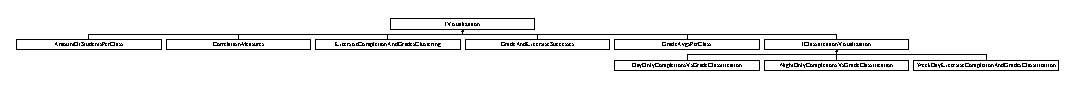
\includegraphics[height=0.727273cm]{classIVisualization}
\end{center}
\end{figure}
\subsection*{Public Member Functions}
\begin{DoxyCompactItemize}
\item 
\mbox{\Hypertarget{classIVisualization_a425d9ec81e192e1264a2b716698449cb}\label{classIVisualization_a425d9ec81e192e1264a2b716698449cb}} 
virtual std\+::string {\bfseries get\+Visualization\+As\+J\+S\+ON} ()=0
\end{DoxyCompactItemize}


The documentation for this class was generated from the following file\+:\begin{DoxyCompactItemize}
\item 
Data\+Processer/src/\+Statistical\+Analyzer/\+Visualizations/I\+Visualization.\+h\end{DoxyCompactItemize}

\hypertarget{classJSONEncoder}{}\section{J\+S\+O\+N\+Encoder Class Reference}
\label{classJSONEncoder}\index{J\+S\+O\+N\+Encoder@{J\+S\+O\+N\+Encoder}}
\subsection*{Public Member Functions}
\begin{DoxyCompactItemize}
\item 
\mbox{\Hypertarget{classJSONEncoder_a617c19c9745055c54b62839b43993148}\label{classJSONEncoder_a617c19c9745055c54b62839b43993148}} 
{\footnotesize template$<$class T , class J $>$ }\\std\+::string {\bfseries pairs\+To\+Json} (std\+::vector$<$ pair$<$ T, J $>$$>$ \&pairs)
\item 
\mbox{\Hypertarget{classJSONEncoder_ae23d931048cc9826daecc247f394bd2a}\label{classJSONEncoder_ae23d931048cc9826daecc247f394bd2a}} 
{\footnotesize template$<$class T , class J $>$ }\\std\+::string {\bfseries map\+To\+Json} (std\+::map$<$ T, J $>$ \&m, bool separate\+Into\+XY)
\item 
\mbox{\Hypertarget{classJSONEncoder_a2dd29be303702a064dd34cf2c811179a}\label{classJSONEncoder_a2dd29be303702a064dd34cf2c811179a}} 
{\footnotesize template$<$class T , class J , class L $>$ }\\std\+::string {\bfseries map\+To\+Json} (std\+::map$<$ T, pair$<$ J, L $>$$>$ \&map\+Of\+Pairs)
\end{DoxyCompactItemize}
\subsection*{Static Public Member Functions}
\begin{DoxyCompactItemize}
\item 
\mbox{\Hypertarget{classJSONEncoder_a7afe6bc64e5edf4a92b7699575da55eb}\label{classJSONEncoder_a7afe6bc64e5edf4a92b7699575da55eb}} 
{\footnotesize template$<$typename T , typename J $>$ }\\static std\+::string {\bfseries pair\+To\+Json} (pair$<$ T, J $>$ \&pair)
\item 
\mbox{\Hypertarget{classJSONEncoder_a892c911683f18153e4e50d1354bb880c}\label{classJSONEncoder_a892c911683f18153e4e50d1354bb880c}} 
{\footnotesize template$<$typename T , typename J $>$ }\\static std\+::string {\bfseries pairs\+To\+Json} (vector$<$ pair$<$ T, J $>$$>$ \&pair\+List)
\item 
\mbox{\Hypertarget{classJSONEncoder_a7d121012e7cf6a5ca957f6325a84074d}\label{classJSONEncoder_a7d121012e7cf6a5ca957f6325a84074d}} 
{\footnotesize template$<$typename T , typename J $>$ }\\static std\+::string {\bfseries map\+To\+Json} (map$<$ T, J $>$ \&map, bool separate\+Into\+XY)
\item 
\mbox{\Hypertarget{classJSONEncoder_ab60fbd11a4b7744bae8e859b2aeaa6d3}\label{classJSONEncoder_ab60fbd11a4b7744bae8e859b2aeaa6d3}} 
{\footnotesize template$<$typename T , typename J , typename L $>$ }\\static std\+::string {\bfseries map\+To\+Json} (map$<$ T, pair$<$ J, L $>$$>$ \&map\+Of\+Pairs)
\item 
\mbox{\Hypertarget{classJSONEncoder_aeb8662e05b14151c6b5bbe07d2eef124}\label{classJSONEncoder_aeb8662e05b14151c6b5bbe07d2eef124}} 
static std\+::string {\bfseries clusters\+To\+J\+S\+ON} (vector$<$ vector$<$ std\+::shared\+\_\+ptr$<$ \hyperlink{classIClusteringPoint}{I\+Clustering\+Point} $>$$>$$>$ clusters)
\end{DoxyCompactItemize}


The documentation for this class was generated from the following files\+:\begin{DoxyCompactItemize}
\item 
Data\+Processer/src/\+Utilities/J\+S\+O\+N\+Encoder.\+h\item 
Data\+Processer/src/\+Utilities/J\+S\+O\+N\+Encoder.\+cpp\item 
Data\+Processer/src/\+Utilities/J\+S\+O\+N\+Encoder.\+inl\end{DoxyCompactItemize}

\hypertarget{classKMeansController}{}\section{K\+Means\+Controller Class Reference}
\label{classKMeansController}\index{K\+Means\+Controller@{K\+Means\+Controller}}
\subsection*{Public Member Functions}
\begin{DoxyCompactItemize}
\item 
\mbox{\Hypertarget{classKMeansController_ae8d2e164feb89f8f6501d0f57309eda1}\label{classKMeansController_ae8d2e164feb89f8f6501d0f57309eda1}} 
{\bfseries K\+Means\+Controller} (vector$<$ shared\+\_\+ptr$<$ \hyperlink{classKMeansPoint}{K\+Means\+Point} $>$$>$ p, int k, int c, int d)
\item 
\mbox{\Hypertarget{classKMeansController_aac8c187bc425b58780e25dadecb710f9}\label{classKMeansController_aac8c187bc425b58780e25dadecb710f9}} 
void {\bfseries run} ()
\item 
\mbox{\Hypertarget{classKMeansController_a7906053fb37cc9184d9d9ecdd1b1bbc4}\label{classKMeansController_a7906053fb37cc9184d9d9ecdd1b1bbc4}} 
vector$<$ vector$<$ shared\+\_\+ptr$<$ \hyperlink{classIClusteringPoint}{I\+Clustering\+Point} $>$ $>$ $>$ {\bfseries get\+Final\+Non\+Empty\+Clusters} ()
\end{DoxyCompactItemize}


The documentation for this class was generated from the following files\+:\begin{DoxyCompactItemize}
\item 
Data\+Processer/src/\+Statistical\+Analyzer/\+K\+Means/K\+Means\+Controller.\+h\item 
Data\+Processer/src/\+Statistical\+Analyzer/\+K\+Means/K\+Means\+Controller.\+cpp\end{DoxyCompactItemize}

\hypertarget{classKMeansIteration}{}\section{K\+Means\+Iteration Class Reference}
\label{classKMeansIteration}\index{K\+Means\+Iteration@{K\+Means\+Iteration}}
\subsection*{Public Member Functions}
\begin{DoxyCompactItemize}
\item 
\mbox{\Hypertarget{classKMeansIteration_ae7a7ca3c1427be0969b5288548c41276}\label{classKMeansIteration_ae7a7ca3c1427be0969b5288548c41276}} 
{\bfseries K\+Means\+Iteration} (vector$<$ \hyperlink{classKMeansPoint}{K\+Means\+Point} $>$ \&p, int \&c, int \&i, int \&d)
\item 
\mbox{\Hypertarget{classKMeansIteration_a435bf71c49dbc0bd497a1992eb1baf57}\label{classKMeansIteration_a435bf71c49dbc0bd497a1992eb1baf57}} 
void {\bfseries run\+Iteration} ()
\end{DoxyCompactItemize}
\subsection*{Public Attributes}
\begin{DoxyCompactItemize}
\item 
\mbox{\Hypertarget{classKMeansIteration_a2ba45f8286e6058129d67fe19df9f0e1}\label{classKMeansIteration_a2ba45f8286e6058129d67fe19df9f0e1}} 
int {\bfseries iteration\+Id}
\item 
\mbox{\Hypertarget{classKMeansIteration_a1923907afbb2aead6b207b9a83998599}\label{classKMeansIteration_a1923907afbb2aead6b207b9a83998599}} 
float {\bfseries sum\+Of\+Squared\+Errors}
\item 
\mbox{\Hypertarget{classKMeansIteration_a7feea077fbea8ad241a42d924e0f8cc7}\label{classKMeansIteration_a7feea077fbea8ad241a42d924e0f8cc7}} 
vector$<$ \hyperlink{classKMeansPoint}{K\+Means\+Point} $>$ \& {\bfseries points}
\end{DoxyCompactItemize}


The documentation for this class was generated from the following files\+:\begin{DoxyCompactItemize}
\item 
Data\+Processer/src/\+Statistical\+Analyzer/\+K\+Means/K\+Means\+Iteration.\+h\item 
Data\+Processer/src/\+Statistical\+Analyzer/\+K\+Means/K\+Means\+Iteration.\+cpp\end{DoxyCompactItemize}

\hypertarget{classKMeansPoint}{}\section{K\+Means\+Point Class Reference}
\label{classKMeansPoint}\index{K\+Means\+Point@{K\+Means\+Point}}
Inheritance diagram for K\+Means\+Point\+:\begin{figure}[H]
\begin{center}
\leavevmode
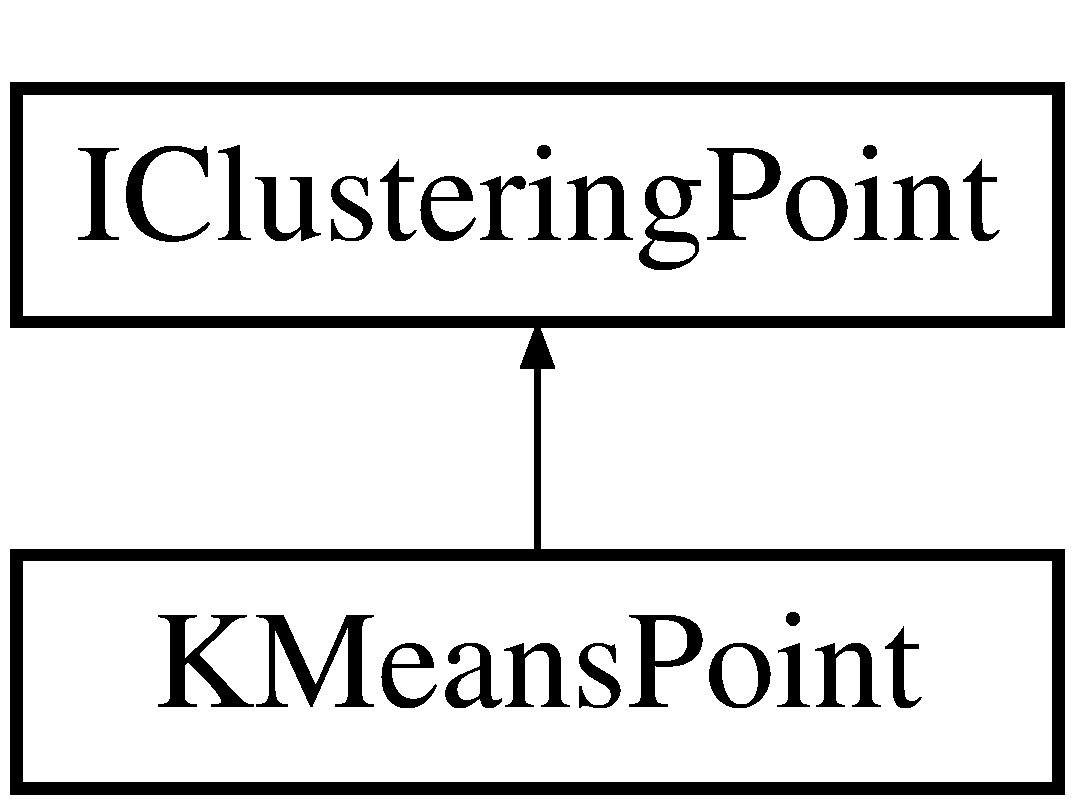
\includegraphics[height=2.000000cm]{classKMeansPoint}
\end{center}
\end{figure}
\subsection*{Public Member Functions}
\begin{DoxyCompactItemize}
\item 
\mbox{\Hypertarget{classKMeansPoint_aa4656fff49410b33987055431ba58083}\label{classKMeansPoint_aa4656fff49410b33987055431ba58083}} 
\hyperlink{classGenericVector}{Generic\+Vector} {\bfseries get\+Vector} () const
\item 
\mbox{\Hypertarget{classKMeansPoint_a2850a53998048945705a3262d836f153}\label{classKMeansPoint_a2850a53998048945705a3262d836f153}} 
int {\bfseries get\+Cluster\+Id} () const
\item 
\mbox{\Hypertarget{classKMeansPoint_a0a83a5f8ffa1b94b0f0e4dc4511ef940}\label{classKMeansPoint_a0a83a5f8ffa1b94b0f0e4dc4511ef940}} 
void {\bfseries set\+Vector} (\hyperlink{classGenericVector}{Generic\+Vector} new\+Vector)
\item 
\mbox{\Hypertarget{classKMeansPoint_a4de80f3770990f507f226fe11764e19f}\label{classKMeansPoint_a4de80f3770990f507f226fe11764e19f}} 
void {\bfseries set\+Cluster\+Id} (int new\+Centroid\+Id)
\item 
\mbox{\Hypertarget{classKMeansPoint_adf92a609a1b137a18026bf4bffe1938f}\label{classKMeansPoint_adf92a609a1b137a18026bf4bffe1938f}} 
{\bfseries K\+Means\+Point} (int c\+Id, \hyperlink{classGenericVector}{Generic\+Vector} gv)
\end{DoxyCompactItemize}
\subsection*{Public Attributes}
\begin{DoxyCompactItemize}
\item 
\mbox{\Hypertarget{classKMeansPoint_ac0d5896b28a976d3bd362b97c120fc18}\label{classKMeansPoint_ac0d5896b28a976d3bd362b97c120fc18}} 
\hyperlink{classGenericVector}{Generic\+Vector} {\bfseries vector}
\item 
\mbox{\Hypertarget{classKMeansPoint_abe666a20a19553a8b37ae038e4cb233a}\label{classKMeansPoint_abe666a20a19553a8b37ae038e4cb233a}} 
int {\bfseries centroid\+Id}
\item 
\mbox{\Hypertarget{classKMeansPoint_a91518c65de711345cefd4f3fcc341471}\label{classKMeansPoint_a91518c65de711345cefd4f3fcc341471}} 
double {\bfseries distance\+To\+Centroid}
\end{DoxyCompactItemize}


The documentation for this class was generated from the following file\+:\begin{DoxyCompactItemize}
\item 
Data\+Processer/src/\+Statistical\+Analyzer/\+Point/K\+Means\+Point.\+h\end{DoxyCompactItemize}

\hypertarget{classKNearestNeighbours}{}\section{K\+Nearest\+Neighbours Class Reference}
\label{classKNearestNeighbours}\index{K\+Nearest\+Neighbours@{K\+Nearest\+Neighbours}}
Inheritance diagram for K\+Nearest\+Neighbours\+:\begin{figure}[H]
\begin{center}
\leavevmode
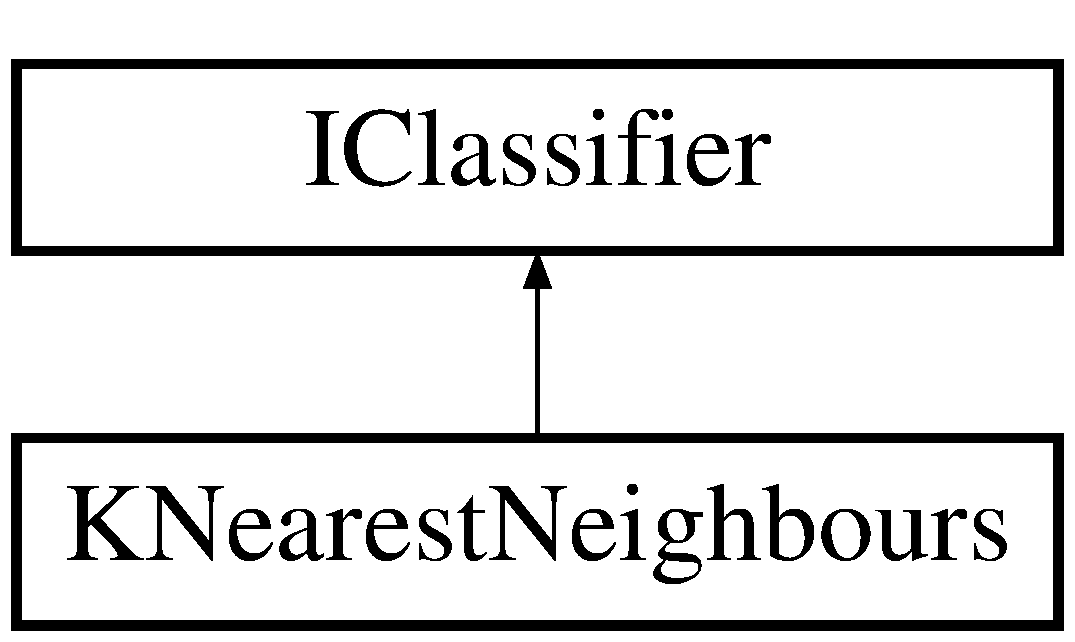
\includegraphics[height=2.000000cm]{classKNearestNeighbours}
\end{center}
\end{figure}
\subsection*{Public Member Functions}
\begin{DoxyCompactItemize}
\item 
\mbox{\Hypertarget{classKNearestNeighbours_a7c479602bf4f949916345ec39a96ea82}\label{classKNearestNeighbours_a7c479602bf4f949916345ec39a96ea82}} 
std\+::vector$<$ std\+::vector$<$ std\+::shared\+\_\+ptr$<$ \hyperlink{classIClusteringPoint}{I\+Clustering\+Point} $>$ $>$ $>$ {\bfseries get\+Classified\+Points} ()
\item 
\mbox{\Hypertarget{classKNearestNeighbours_a22bd79b738fe1af311586dfc1bb311bf}\label{classKNearestNeighbours_a22bd79b738fe1af311586dfc1bb311bf}} 
void {\bfseries initialize} (std\+::vector$<$ std\+::shared\+\_\+ptr$<$ \hyperlink{classIClusteringPoint}{I\+Clustering\+Point} $>$$>$ input, vector$<$ vector$<$ std\+::shared\+\_\+ptr$<$ \hyperlink{classIClusteringPoint}{I\+Clustering\+Point} $>$$>$$>$ tc)
\end{DoxyCompactItemize}
\subsection*{Static Public Member Functions}
\begin{DoxyCompactItemize}
\item 
\mbox{\Hypertarget{classKNearestNeighbours_a5c9ecb63d9e5f61789b417c363a27bd8}\label{classKNearestNeighbours_a5c9ecb63d9e5f61789b417c363a27bd8}} 
static std\+::vector$<$ std\+::shared\+\_\+ptr$<$ \hyperlink{classIClusteringPoint}{I\+Clustering\+Point} $>$ $>$ {\bfseries get\+Nearest\+Neighbours} (std\+::shared\+\_\+ptr$<$ \hyperlink{classIClusteringPoint}{I\+Clustering\+Point} $>$ \&point, int max\+Amount\+Of\+Neighbours, std\+::vector$<$ std\+::vector$<$ std\+::shared\+\_\+ptr$<$ \hyperlink{classIClusteringPoint}{I\+Clustering\+Point} $>$$>$$>$ \&clusters)
\end{DoxyCompactItemize}


The documentation for this class was generated from the following files\+:\begin{DoxyCompactItemize}
\item 
Data\+Processer/src/\+Statistical\+Analyzer/\+Classifiers/\+K\+Nearest\+Neighbours/K\+Nearest\+Neighbours.\+h\item 
Data\+Processer/src/\+Statistical\+Analyzer/\+Classifiers/\+K\+Nearest\+Neighbours/K\+Nearest\+Neighbours.\+cpp\end{DoxyCompactItemize}

\hypertarget{classLogarithmicLinearRegression}{}\section{Logarithmic\+Linear\+Regression Class Reference}
\label{classLogarithmicLinearRegression}\index{Logarithmic\+Linear\+Regression@{Logarithmic\+Linear\+Regression}}
Inheritance diagram for Logarithmic\+Linear\+Regression\+:\begin{figure}[H]
\begin{center}
\leavevmode
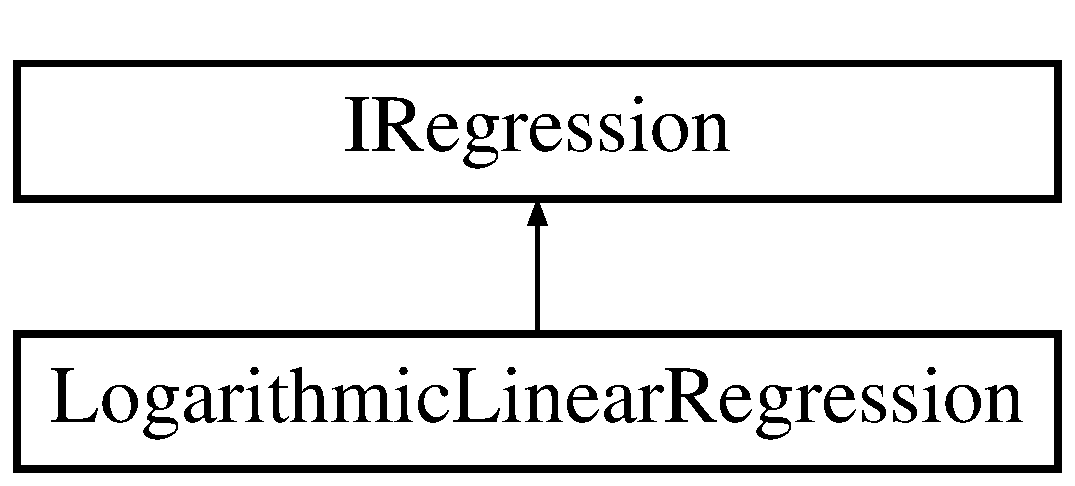
\includegraphics[height=2.000000cm]{classLogarithmicLinearRegression}
\end{center}
\end{figure}
\subsection*{Public Member Functions}
\begin{DoxyCompactItemize}
\item 
\mbox{\Hypertarget{classLogarithmicLinearRegression_ad1a7402c328c6ed416a5512a3c2de429}\label{classLogarithmicLinearRegression_ad1a7402c328c6ed416a5512a3c2de429}} 
std\+::string {\bfseries get\+Regression\+As\+J\+S\+ON} ()
\item 
\mbox{\Hypertarget{classLogarithmicLinearRegression_a52f142e314972005fec7c29f967d285a}\label{classLogarithmicLinearRegression_a52f142e314972005fec7c29f967d285a}} 
{\bfseries Logarithmic\+Linear\+Regression} (std\+::vector$<$ std\+::pair$<$ float, float $>$$>$ p)
\end{DoxyCompactItemize}
\subsection*{Protected Member Functions}
\begin{DoxyCompactItemize}
\item 
\mbox{\Hypertarget{classLogarithmicLinearRegression_a83d205c11fbd5e213b6c9d1001347c0d}\label{classLogarithmicLinearRegression_a83d205c11fbd5e213b6c9d1001347c0d}} 
float {\bfseries get\+Slope} ()
\item 
\mbox{\Hypertarget{classLogarithmicLinearRegression_a2d200638d2a95e86a445d4f318a2f6c6}\label{classLogarithmicLinearRegression_a2d200638d2a95e86a445d4f318a2f6c6}} 
float {\bfseries get\+Intercept} ()
\item 
\mbox{\Hypertarget{classLogarithmicLinearRegression_ad74d3d4fea7588caa8cf0df3b633a842}\label{classLogarithmicLinearRegression_ad74d3d4fea7588caa8cf0df3b633a842}} 
std\+::vector$<$ std\+::pair$<$ float, float $>$ $>$ {\bfseries get\+Regression} ()
\end{DoxyCompactItemize}
\subsection*{Additional Inherited Members}


The documentation for this class was generated from the following files\+:\begin{DoxyCompactItemize}
\item 
Data\+Processer/src/\+Statistical\+Analyzer/\+Regression/Logarithmic\+Linear\+Regression.\+h\item 
Data\+Processer/src/\+Statistical\+Analyzer/\+Regression/Logarithmic\+Linear\+Regression.\+cpp\end{DoxyCompactItemize}

\hypertarget{classMapper}{}\section{Mapper Class Reference}
\label{classMapper}\index{Mapper@{Mapper}}
\subsection*{Public Member Functions}
\begin{DoxyCompactItemize}
\item 
\mbox{\Hypertarget{classMapper_af544846befd0cad6dfd62667224f2443}\label{classMapper_af544846befd0cad6dfd62667224f2443}} 
{\bfseries Mapper} (vector$<$ \hyperlink{classYamlObject}{Yaml\+Object} $>$ \&email\+Yaml, vector$<$ \hyperlink{classYamlObject}{Yaml\+Object} $>$ \&anonymous\+Yaml, vector$<$ vector$<$ string $>$$>$ \&class\+Emails)
\item 
\mbox{\Hypertarget{classMapper_a93e9f23580b940a5a9d01abaa772163e}\label{classMapper_a93e9f23580b940a5a9d01abaa772163e}} 
void {\bfseries create\+Yaml\+Files\+With\+Classes} ()
\item 
\mbox{\Hypertarget{classMapper_a8c097d98de06d34199ab1409a9598515}\label{classMapper_a8c097d98de06d34199ab1409a9598515}} 
void {\bfseries create\+Grades\+Yaml\+File} (ofstream \&outfile)
\item 
\mbox{\Hypertarget{classMapper_a95d637dc7c5ef852920852167675cd00}\label{classMapper_a95d637dc7c5ef852920852167675cd00}} 
void {\bfseries create\+Yaml\+File\+From\+Map} (map$<$ string, string $>$ \&keys\+And\+Values, string identifier\+Key)
\end{DoxyCompactItemize}


The documentation for this class was generated from the following files\+:\begin{DoxyCompactItemize}
\item 
Data\+Processer/src/\+Mapper/Mapper.\+h\item 
Data\+Processer/src/\+Mapper/Mapper.\+cpp\end{DoxyCompactItemize}

\hypertarget{classNaiveBayesClassification}{}\section{Naive\+Bayes\+Classification Class Reference}
\label{classNaiveBayesClassification}\index{Naive\+Bayes\+Classification@{Naive\+Bayes\+Classification}}
Inheritance diagram for Naive\+Bayes\+Classification\+:\begin{figure}[H]
\begin{center}
\leavevmode
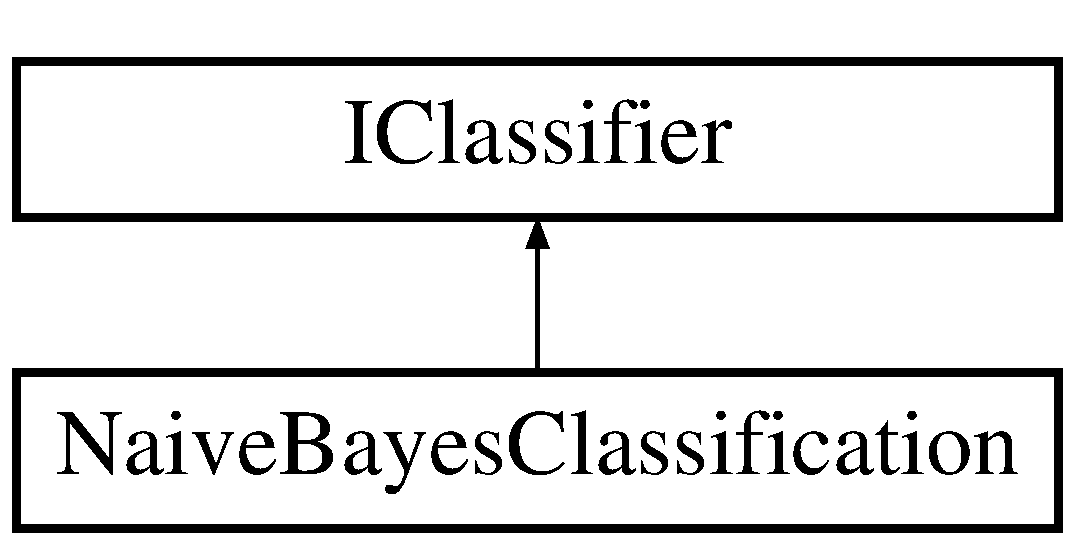
\includegraphics[height=2.000000cm]{classNaiveBayesClassification}
\end{center}
\end{figure}
\subsection*{Public Member Functions}
\begin{DoxyCompactItemize}
\item 
\mbox{\Hypertarget{classNaiveBayesClassification_a3d6e4ab088b7cb6a310270e5b6fc86ae}\label{classNaiveBayesClassification_a3d6e4ab088b7cb6a310270e5b6fc86ae}} 
std\+::vector$<$ std\+::vector$<$ std\+::shared\+\_\+ptr$<$ \hyperlink{classIClusteringPoint}{I\+Clustering\+Point} $>$ $>$ $>$ {\bfseries get\+Classified\+Points} ()
\item 
\mbox{\Hypertarget{classNaiveBayesClassification_a17cb800221babf87be8b188b25de198b}\label{classNaiveBayesClassification_a17cb800221babf87be8b188b25de198b}} 
void {\bfseries initialize} (std\+::vector$<$ std\+::shared\+\_\+ptr$<$ \hyperlink{classIClusteringPoint}{I\+Clustering\+Point} $>$$>$ input, vector$<$ vector$<$ std\+::shared\+\_\+ptr$<$ \hyperlink{classIClusteringPoint}{I\+Clustering\+Point} $>$$>$$>$ trainingset)
\end{DoxyCompactItemize}


The documentation for this class was generated from the following files\+:\begin{DoxyCompactItemize}
\item 
Data\+Processer/src/\+Statistical\+Analyzer/\+Classifiers/\+Naive\+Bayes\+Classification/Naive\+Bayes\+Classification.\+h\item 
Data\+Processer/src/\+Statistical\+Analyzer/\+Classifiers/\+Naive\+Bayes\+Classification/Naive\+Bayes\+Classification.\+cpp\end{DoxyCompactItemize}

\hypertarget{classNightOnlyCompletionsVsGradeClassification}{}\section{Night\+Only\+Completions\+Vs\+Grade\+Classification Class Reference}
\label{classNightOnlyCompletionsVsGradeClassification}\index{Night\+Only\+Completions\+Vs\+Grade\+Classification@{Night\+Only\+Completions\+Vs\+Grade\+Classification}}
Inheritance diagram for Night\+Only\+Completions\+Vs\+Grade\+Classification\+:\begin{figure}[H]
\begin{center}
\leavevmode
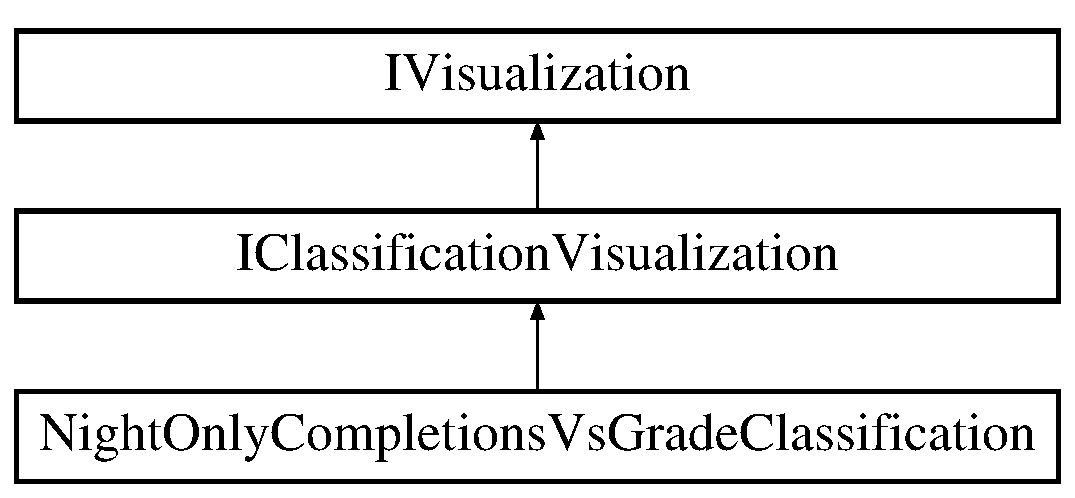
\includegraphics[height=3.000000cm]{classNightOnlyCompletionsVsGradeClassification}
\end{center}
\end{figure}
\subsection*{Public Member Functions}
\begin{DoxyCompactItemize}
\item 
\mbox{\Hypertarget{classNightOnlyCompletionsVsGradeClassification_a1f821edac48f28cd19d691bed21e41a3}\label{classNightOnlyCompletionsVsGradeClassification_a1f821edac48f28cd19d691bed21e41a3}} 
{\bfseries Night\+Only\+Completions\+Vs\+Grade\+Classification} (std\+::shared\+\_\+ptr$<$ \hyperlink{classIClassifier}{I\+Classifier} $>$ cl, std\+::shared\+\_\+ptr$<$ \hyperlink{classIFilter}{I\+Filter} $>$ gf, std\+::shared\+\_\+ptr$<$ \hyperlink{classIFilter}{I\+Filter} $>$ af)
\end{DoxyCompactItemize}


The documentation for this class was generated from the following files\+:\begin{DoxyCompactItemize}
\item 
Data\+Processer/src/\+Statistical\+Analyzer/\+Visualizations/Night\+Only\+Completions\+Vs\+Grade\+Classification.\+h\item 
Data\+Processer/src/\+Statistical\+Analyzer/\+Visualizations/Night\+Only\+Completions\+Vs\+Grade\+Classification.\+cpp\end{DoxyCompactItemize}

\hypertarget{classNightOnlyFilter}{}\section{Night\+Only\+Filter Class Reference}
\label{classNightOnlyFilter}\index{Night\+Only\+Filter@{Night\+Only\+Filter}}
Inheritance diagram for Night\+Only\+Filter\+:\begin{figure}[H]
\begin{center}
\leavevmode
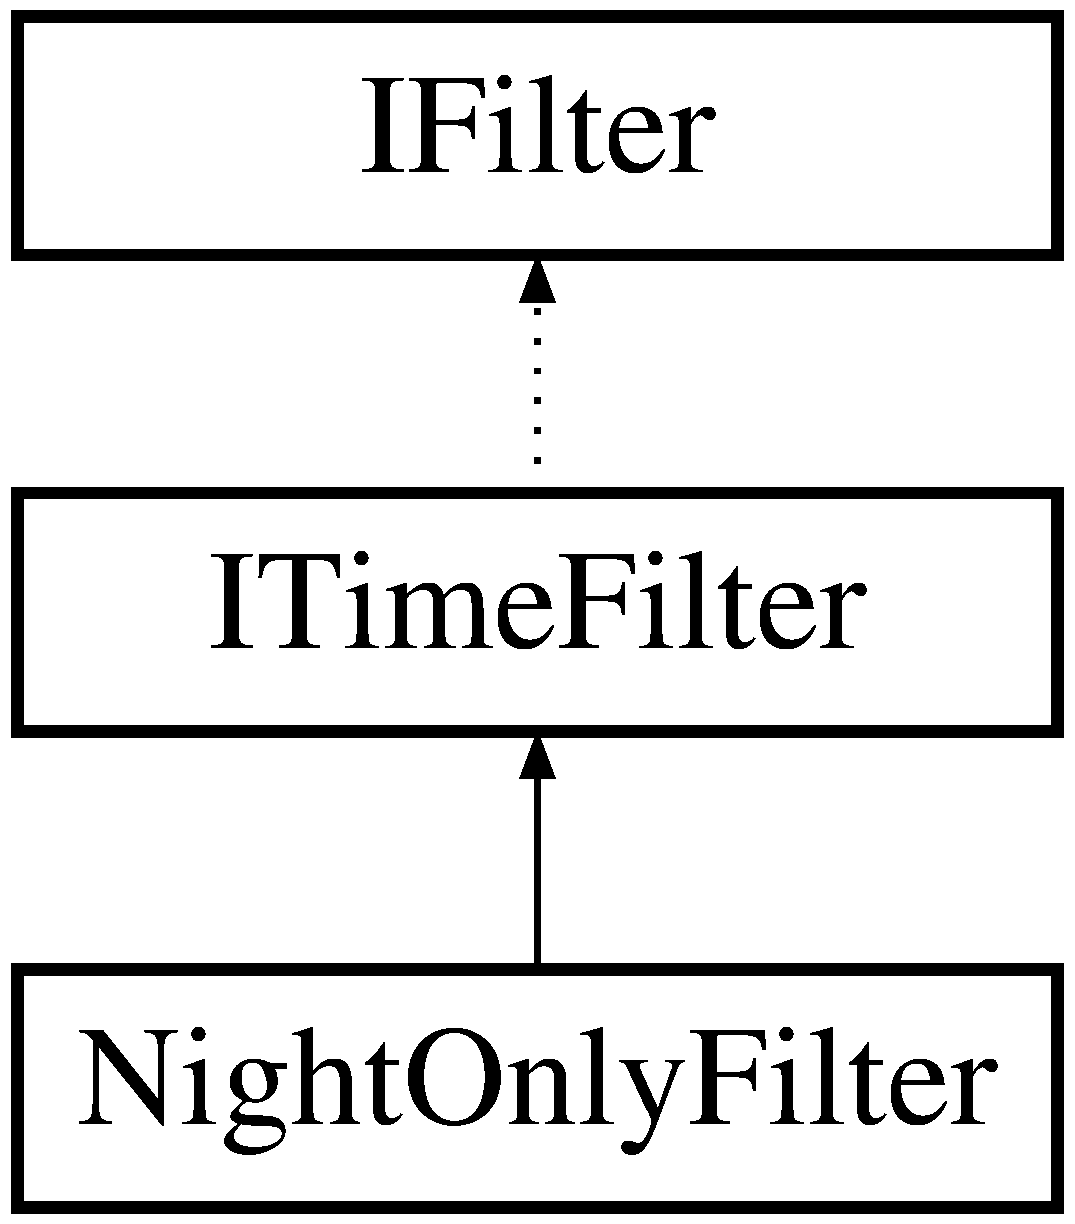
\includegraphics[height=3.000000cm]{classNightOnlyFilter}
\end{center}
\end{figure}
\subsection*{Public Member Functions}
\begin{DoxyCompactItemize}
\item 
\mbox{\Hypertarget{classNightOnlyFilter_a10071792de61a025fb3416b2e3a0da9d}\label{classNightOnlyFilter_a10071792de61a025fb3416b2e3a0da9d}} 
void {\bfseries set\+Filter\+Query\+Column\+Indexes} (\hyperlink{structFilterQueryColumnIndexes}{Filter\+Query\+Column\+Indexes} fq)
\item 
\mbox{\Hypertarget{classNightOnlyFilter_a8efc92bd9d61b15700141db8d8687f53}\label{classNightOnlyFilter_a8efc92bd9d61b15700141db8d8687f53}} 
\hyperlink{structFilterQueryColumnIndexes}{Filter\+Query\+Column\+Indexes} {\bfseries get\+Filter\+Query\+Column\+Indexes} ()
\end{DoxyCompactItemize}
\subsection*{Public Attributes}
\begin{DoxyCompactItemize}
\item 
\mbox{\Hypertarget{classNightOnlyFilter_a5411878df9e064072f750b7cf26286ae}\label{classNightOnlyFilter_a5411878df9e064072f750b7cf26286ae}} 
\hyperlink{structFilterQueryColumnIndexes}{Filter\+Query\+Column\+Indexes} {\bfseries query\+Column\+Indexes}
\end{DoxyCompactItemize}


The documentation for this class was generated from the following files\+:\begin{DoxyCompactItemize}
\item 
Data\+Processer/src/\+Statistical\+Analyzer/\+Filter/Night\+Only\+Filter.\+h\item 
Data\+Processer/src/\+Statistical\+Analyzer/\+Filter/Night\+Only\+Filter.\+cpp\end{DoxyCompactItemize}

\hypertarget{classSimpleLinearRegression}{}\section{Simple\+Linear\+Regression Class Reference}
\label{classSimpleLinearRegression}\index{Simple\+Linear\+Regression@{Simple\+Linear\+Regression}}
Inheritance diagram for Simple\+Linear\+Regression\+:\begin{figure}[H]
\begin{center}
\leavevmode
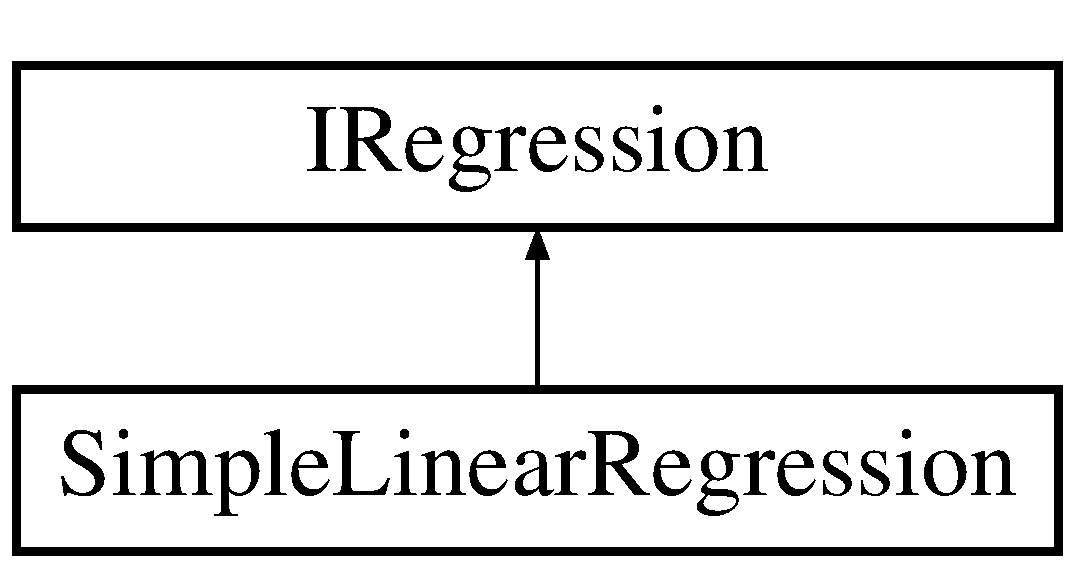
\includegraphics[height=2.000000cm]{classSimpleLinearRegression}
\end{center}
\end{figure}
\subsection*{Public Member Functions}
\begin{DoxyCompactItemize}
\item 
\mbox{\Hypertarget{classSimpleLinearRegression_a920bc4a7c09c08662ca4b44b7b2e0782}\label{classSimpleLinearRegression_a920bc4a7c09c08662ca4b44b7b2e0782}} 
std\+::string {\bfseries get\+Regression\+As\+J\+S\+ON} ()
\item 
\mbox{\Hypertarget{classSimpleLinearRegression_aa37166df3d358d5c1a96b48c0f9c41af}\label{classSimpleLinearRegression_aa37166df3d358d5c1a96b48c0f9c41af}} 
{\bfseries Simple\+Linear\+Regression} (std\+::vector$<$ std\+::pair$<$ float, float $>$$>$ p)
\end{DoxyCompactItemize}
\subsection*{Protected Member Functions}
\begin{DoxyCompactItemize}
\item 
\mbox{\Hypertarget{classSimpleLinearRegression_a6e5edd1518c4b0b1d5bd6f1db30c14d4}\label{classSimpleLinearRegression_a6e5edd1518c4b0b1d5bd6f1db30c14d4}} 
float {\bfseries get\+Slope} ()
\item 
\mbox{\Hypertarget{classSimpleLinearRegression_a3b30ccdf0d57eef38aa44e98588dc14f}\label{classSimpleLinearRegression_a3b30ccdf0d57eef38aa44e98588dc14f}} 
float {\bfseries get\+Intercept} ()
\item 
\mbox{\Hypertarget{classSimpleLinearRegression_ae61271a16954d19c0cc8a5d2b7006c3d}\label{classSimpleLinearRegression_ae61271a16954d19c0cc8a5d2b7006c3d}} 
std\+::vector$<$ std\+::pair$<$ float, float $>$ $>$ {\bfseries get\+Regression} ()
\end{DoxyCompactItemize}
\subsection*{Additional Inherited Members}


The documentation for this class was generated from the following files\+:\begin{DoxyCompactItemize}
\item 
Data\+Processer/src/\+Statistical\+Analyzer/\+Regression/Simple\+Linear\+Regression.\+h\item 
Data\+Processer/src/\+Statistical\+Analyzer/\+Regression/Simple\+Linear\+Regression.\+cpp\end{DoxyCompactItemize}

\hypertarget{classSimpleLinearRegressionTest}{}\section{Simple\+Linear\+Regression\+Test Class Reference}
\label{classSimpleLinearRegressionTest}\index{Simple\+Linear\+Regression\+Test@{Simple\+Linear\+Regression\+Test}}
Inheritance diagram for Simple\+Linear\+Regression\+Test\+:\begin{figure}[H]
\begin{center}
\leavevmode
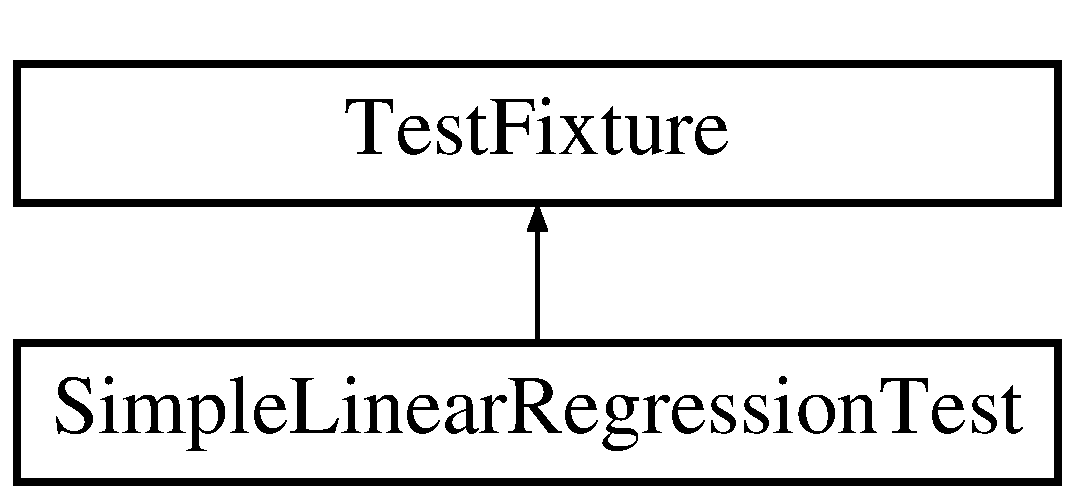
\includegraphics[height=2.000000cm]{classSimpleLinearRegressionTest}
\end{center}
\end{figure}
\subsection*{Public Member Functions}
\begin{DoxyCompactItemize}
\item 
\mbox{\Hypertarget{classSimpleLinearRegressionTest_a4330926babb43ab5e40c66902a8401c5}\label{classSimpleLinearRegressionTest_a4330926babb43ab5e40c66902a8401c5}} 
void {\bfseries test\+Intercept} ()
\item 
\mbox{\Hypertarget{classSimpleLinearRegressionTest_a9de5a17b46e2a0370366698fe63e7c6a}\label{classSimpleLinearRegressionTest_a9de5a17b46e2a0370366698fe63e7c6a}} 
void {\bfseries test\+Slope} ()
\end{DoxyCompactItemize}
\subsection*{Static Public Member Functions}
\begin{DoxyCompactItemize}
\item 
\mbox{\Hypertarget{classSimpleLinearRegressionTest_a82b98fdff3711e204b8f7b47723c43a0}\label{classSimpleLinearRegressionTest_a82b98fdff3711e204b8f7b47723c43a0}} 
static Cpp\+Unit\+::\+Test $\ast$ {\bfseries suite} ()
\end{DoxyCompactItemize}


The documentation for this class was generated from the following file\+:\begin{DoxyCompactItemize}
\item 
Data\+Processer/tests/Simple\+Linear\+Regression\+Test.\+h\end{DoxyCompactItemize}

\hypertarget{classStatisticalToolsTest}{}\section{Statistical\+Tools\+Test Class Reference}
\label{classStatisticalToolsTest}\index{Statistical\+Tools\+Test@{Statistical\+Tools\+Test}}
Inheritance diagram for Statistical\+Tools\+Test\+:\begin{figure}[H]
\begin{center}
\leavevmode
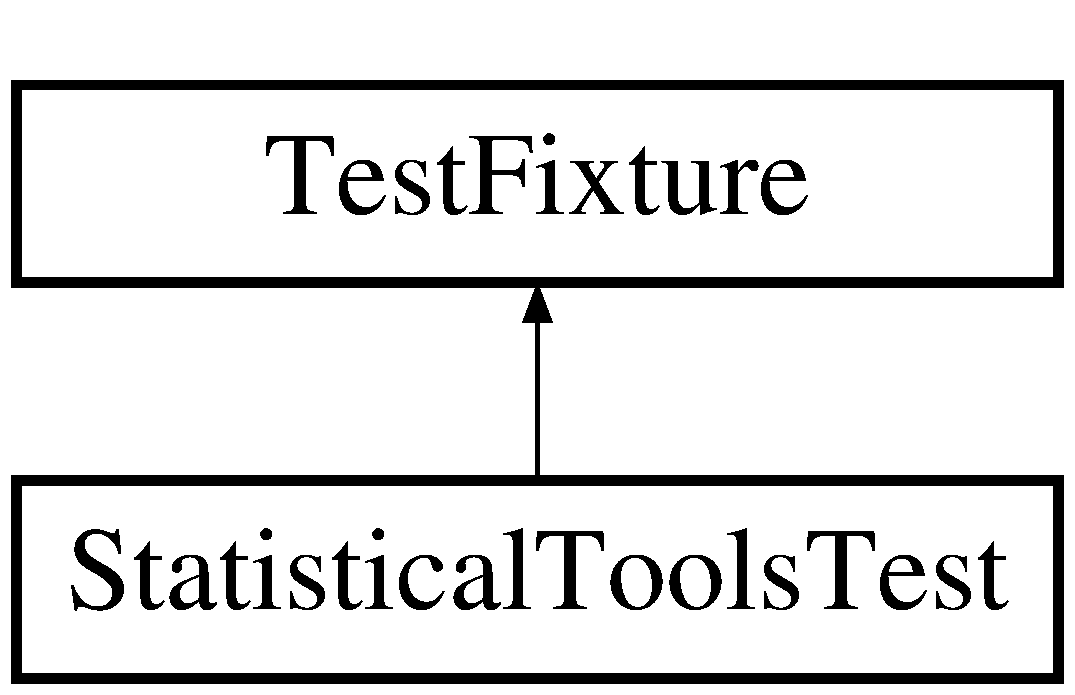
\includegraphics[height=2.000000cm]{classStatisticalToolsTest}
\end{center}
\end{figure}
\subsection*{Public Member Functions}
\begin{DoxyCompactItemize}
\item 
\mbox{\Hypertarget{classStatisticalToolsTest_aa9318bda5f30d8bd4e55d73e2afaeca7}\label{classStatisticalToolsTest_aa9318bda5f30d8bd4e55d73e2afaeca7}} 
void {\bfseries test\+Mean} ()
\item 
\mbox{\Hypertarget{classStatisticalToolsTest_a8aad8e70798d8691cb90658c82069a12}\label{classStatisticalToolsTest_a8aad8e70798d8691cb90658c82069a12}} 
void {\bfseries test\+Standard\+Deviation} ()
\end{DoxyCompactItemize}
\subsection*{Static Public Member Functions}
\begin{DoxyCompactItemize}
\item 
\mbox{\Hypertarget{classStatisticalToolsTest_aa983611e198dba8c31fc572cf0366217}\label{classStatisticalToolsTest_aa983611e198dba8c31fc572cf0366217}} 
static Cpp\+Unit\+::\+Test $\ast$ {\bfseries suite} ()
\end{DoxyCompactItemize}


The documentation for this class was generated from the following files\+:\begin{DoxyCompactItemize}
\item 
Data\+Processer/tests/Statistical\+Tools\+Test.\+h\item 
Data\+Processer/tests/Statistical\+Tools\+Test.\+cpp\end{DoxyCompactItemize}

\hypertarget{classUtcReader}{}\section{Utc\+Reader Class Reference}
\label{classUtcReader}\index{Utc\+Reader@{Utc\+Reader}}
\subsection*{Static Public Member Functions}
\begin{DoxyCompactItemize}
\item 
\mbox{\Hypertarget{classUtcReader_a31a33f96f4beac8f8d91086bd577edd3}\label{classUtcReader_a31a33f96f4beac8f8d91086bd577edd3}} 
static \hyperlink{classUtcTime}{Utc\+Time} {\bfseries to\+Utc\+Time} (std\+::string \&s)
\end{DoxyCompactItemize}


The documentation for this class was generated from the following files\+:\begin{DoxyCompactItemize}
\item 
Data\+Processer/src/\+Utilities/Utc\+Reader.\+h\item 
Data\+Processer/src/\+Utilities/Utc\+Reader.\+cpp\end{DoxyCompactItemize}

\hypertarget{classUtcTime}{}\section{Utc\+Time Class Reference}
\label{classUtcTime}\index{Utc\+Time@{Utc\+Time}}
\subsection*{Public Member Functions}
\begin{DoxyCompactItemize}
\item 
\mbox{\Hypertarget{classUtcTime_a0c7adf939e9c0d25844d1901bdc75a31}\label{classUtcTime_a0c7adf939e9c0d25844d1901bdc75a31}} 
{\bfseries Utc\+Time} (int y, int m, int d, int h, int min, double s)
\item 
\mbox{\Hypertarget{classUtcTime_a51213d81df592f14782853569c150e49}\label{classUtcTime_a51213d81df592f14782853569c150e49}} 
std\+::string {\bfseries To\+String} ()
\end{DoxyCompactItemize}
\subsection*{Public Attributes}
\begin{DoxyCompactItemize}
\item 
\mbox{\Hypertarget{classUtcTime_a8e69cfba3818d7fe34fdb688ee983d49}\label{classUtcTime_a8e69cfba3818d7fe34fdb688ee983d49}} 
int {\bfseries year}
\item 
\mbox{\Hypertarget{classUtcTime_a2594e00e74b015f01eb45f539b1eb214}\label{classUtcTime_a2594e00e74b015f01eb45f539b1eb214}} 
int {\bfseries month}
\item 
\mbox{\Hypertarget{classUtcTime_a6fa8ddb218225c2be962a29c1213037c}\label{classUtcTime_a6fa8ddb218225c2be962a29c1213037c}} 
int {\bfseries day}
\item 
\mbox{\Hypertarget{classUtcTime_af940818b8bc15fa234b11e0f09ac6c19}\label{classUtcTime_af940818b8bc15fa234b11e0f09ac6c19}} 
int {\bfseries hour}
\item 
\mbox{\Hypertarget{classUtcTime_abd0eda4abd006d346ffeadc33a1d10fc}\label{classUtcTime_abd0eda4abd006d346ffeadc33a1d10fc}} 
int {\bfseries minute}
\item 
\mbox{\Hypertarget{classUtcTime_aec1f76c5ce0c2787654713b2fd42c978}\label{classUtcTime_aec1f76c5ce0c2787654713b2fd42c978}} 
double {\bfseries second}
\end{DoxyCompactItemize}


The documentation for this class was generated from the following files\+:\begin{DoxyCompactItemize}
\item 
Data\+Processer/src/\+Utilities/Utc\+Time.\+h\item 
Data\+Processer/src/\+Utilities/Utc\+Time.\+cpp\end{DoxyCompactItemize}

\hypertarget{classUtilities}{}\section{Utilities Class Reference}
\label{classUtilities}\index{Utilities@{Utilities}}
\subsection*{Static Public Member Functions}
\begin{DoxyCompactItemize}
\item 
\mbox{\Hypertarget{classUtilities_a6b05484ec7d0d5a71f4ccd775f20a5c2}\label{classUtilities_a6b05484ec7d0d5a71f4ccd775f20a5c2}} 
static vector$<$ string $>$ {\bfseries get\+List\+Of\+Numbered\+Files\+For\+Base\+File} (string base\+File\+String)
\item 
\mbox{\Hypertarget{classUtilities_a6a2654b7cbbc430b17d42e520159b91e}\label{classUtilities_a6a2654b7cbbc430b17d42e520159b91e}} 
static void {\bfseries remove\+Yaml\+References} (string \&str)
\item 
\mbox{\Hypertarget{classUtilities_ac8923fd8433ca415a895a2298a03a2e7}\label{classUtilities_ac8923fd8433ca415a895a2298a03a2e7}} 
static string {\bfseries create\+Str\+With\+White\+Spaces} (int amount)
\item 
\mbox{\Hypertarget{classUtilities_af0943918d7b3643596ab93ea8333894f}\label{classUtilities_af0943918d7b3643596ab93ea8333894f}} 
static void {\bfseries remove\+Str\+White\+Space} (string \&str)
\item 
\mbox{\Hypertarget{classUtilities_a87920ab569865b8fdb87bc2484ba0fb3}\label{classUtilities_a87920ab569865b8fdb87bc2484ba0fb3}} 
static bool {\bfseries is\+N\+Chars\+White\+Space} (int N, string \&str)
\item 
\mbox{\Hypertarget{classUtilities_a6eb13a9d34f53096f88579523c766a70}\label{classUtilities_a6eb13a9d34f53096f88579523c766a70}} 
static bool {\bfseries Are\+Floats\+Equal} (float f1, float f2)
\item 
\mbox{\Hypertarget{classUtilities_a64040506330ee0342c7ffafbeef76e41}\label{classUtilities_a64040506330ee0342c7ffafbeef76e41}} 
static int {\bfseries compute\+Average} (vector$<$ int $>$ \&values)
\item 
\mbox{\Hypertarget{classUtilities_a32fc9c952880eff1d83929f4b42e75e0}\label{classUtilities_a32fc9c952880eff1d83929f4b42e75e0}} 
static bool {\bfseries is\+In\+Vector} (string \&value, vector$<$ string $>$ \&vector)
\item 
\mbox{\Hypertarget{classUtilities_ac65283ddc58535bf53f9ecc66b71cf85}\label{classUtilities_ac65283ddc58535bf53f9ecc66b71cf85}} 
{\footnotesize template$<$class T , class J $>$ }\\static vector$<$ T $>$ {\bfseries get\+Keys\+Of\+Map} (map$<$ T, J $>$ m)
\item 
\mbox{\Hypertarget{classUtilities_a7e9774c5147408d41ca75e54970e74e2}\label{classUtilities_a7e9774c5147408d41ca75e54970e74e2}} 
{\footnotesize template$<$class T , class J $>$ }\\static vector$<$ J $>$ {\bfseries get\+Values\+Of\+Map} (map$<$ T, J $>$ m)
\item 
\mbox{\Hypertarget{classUtilities_a1770afc90489caae248bbbcac40e71d9}\label{classUtilities_a1770afc90489caae248bbbcac40e71d9}} 
{\footnotesize template$<$class T , class J $>$ }\\static pair$<$ T, J $>$ {\bfseries get\+Highest\+Or\+Lowest\+Value\+KV} (map$<$ T, J $>$ m, bool get\+Highest)
\item 
\mbox{\Hypertarget{classUtilities_a9ad8649d85727540f66adb4c6644c0a1}\label{classUtilities_a9ad8649d85727540f66adb4c6644c0a1}} 
static vector$<$ pqxx\+::result\+::tuple $>$ {\bfseries to\+List\+Of\+Pqxx\+Tuples} (pqxx\+::result \&r)
\item 
\mbox{\Hypertarget{classUtilities_a868b728a68449405c6d65632246ddf42}\label{classUtilities_a868b728a68449405c6d65632246ddf42}} 
{\footnotesize template$<$class T $>$ }\\static string {\bfseries generic\+To\+Str} (const T \&val)
\item 
\mbox{\Hypertarget{classUtilities_a522d29d118f7a72a451b9c6392f24081}\label{classUtilities_a522d29d118f7a72a451b9c6392f24081}} 
static vector$<$ string $>$ {\bfseries to\+Array\+By\+Delim} (string \&s, char delim)
\item 
\mbox{\Hypertarget{classUtilities_a82e8f55c09721bf7d8cd483047f44140}\label{classUtilities_a82e8f55c09721bf7d8cd483047f44140}} 
static vector$<$ std\+::shared\+\_\+ptr$<$ \hyperlink{classIClusteringPoint}{I\+Clustering\+Point} $>$ $>$ {\bfseries convert\+Map\+Of\+Pairs\+To\+Points} (map$<$ string, pair$<$ int, int $>$$>$ input\+Values)
\item 
\mbox{\Hypertarget{classUtilities_a6f03912b65bc19ac2e4c52f42ef970b1}\label{classUtilities_a6f03912b65bc19ac2e4c52f42ef970b1}} 
static vector$<$ std\+::shared\+\_\+ptr$<$ \hyperlink{classKMeansPoint}{K\+Means\+Point} $>$ $>$ {\bfseries convert\+Map\+Of\+Pairs\+To\+K\+Means\+Points} (map$<$ string, pair$<$ int, int $>$$>$ input\+Values)
\item 
\mbox{\Hypertarget{classUtilities_aba6071414ba172e34c2f7e6996b8d5e5}\label{classUtilities_aba6071414ba172e34c2f7e6996b8d5e5}} 
static vector$<$ std\+::shared\+\_\+ptr$<$ \hyperlink{classDBScanPoint}{D\+B\+Scan\+Point} $>$ $>$ {\bfseries convert\+Map\+Of\+Pairs\+To\+D\+B\+Scan\+Points} (map$<$ string, pair$<$ int, int $>$$>$ input\+Values)
\end{DoxyCompactItemize}


The documentation for this class was generated from the following files\+:\begin{DoxyCompactItemize}
\item 
Data\+Processer/src/\+Utilities/Utilities.\+h\item 
Data\+Processer/src/\+Utilities/Utilities.\+cpp\end{DoxyCompactItemize}

\hypertarget{classUtilitiesTest}{}\section{Utilities\+Test Class Reference}
\label{classUtilitiesTest}\index{Utilities\+Test@{Utilities\+Test}}
Inheritance diagram for Utilities\+Test\+:\begin{figure}[H]
\begin{center}
\leavevmode
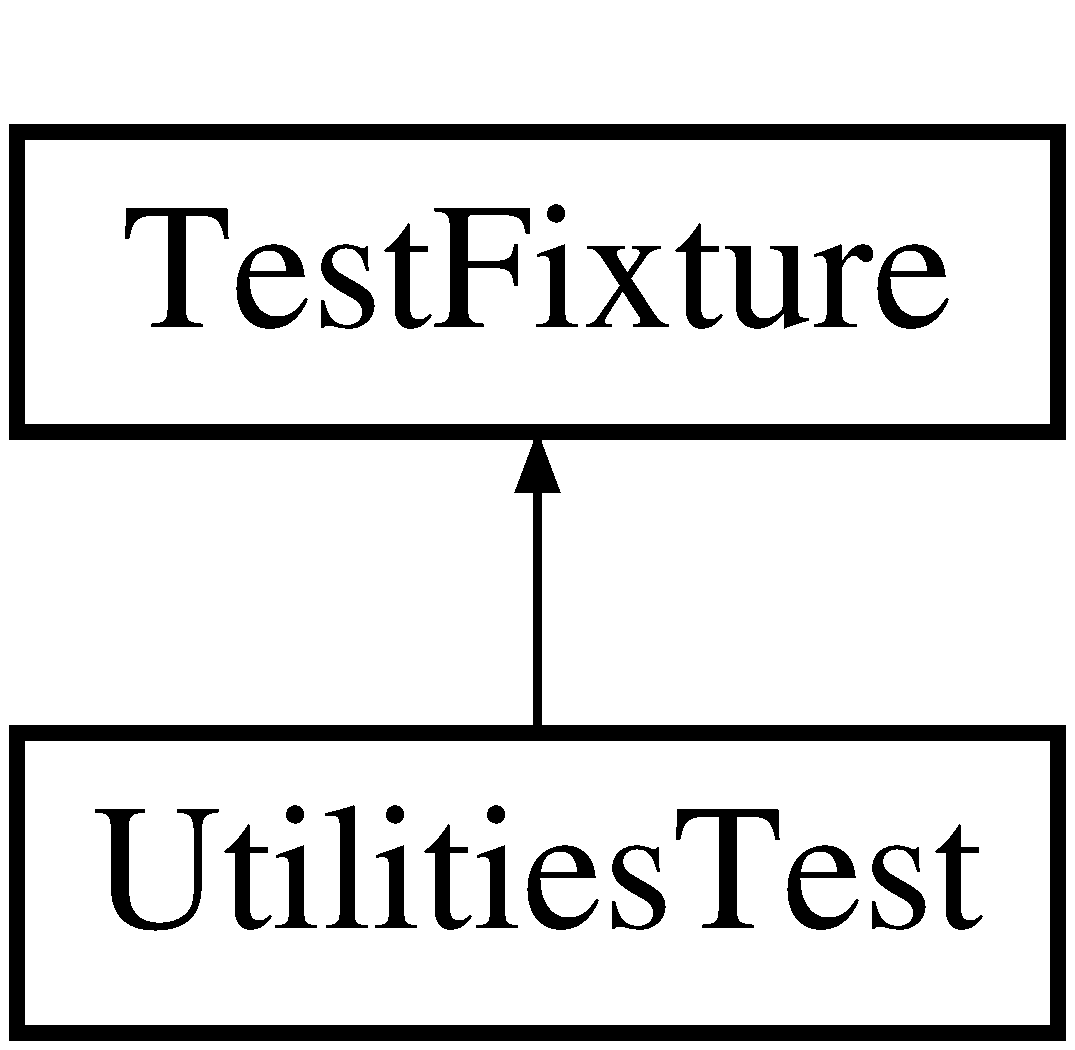
\includegraphics[height=2.000000cm]{classUtilitiesTest}
\end{center}
\end{figure}
\subsection*{Public Member Functions}
\begin{DoxyCompactItemize}
\item 
\mbox{\Hypertarget{classUtilitiesTest_abeeace607b8a06666d96e5951f05342e}\label{classUtilitiesTest_abeeace607b8a06666d96e5951f05342e}} 
void {\bfseries test\+Is\+N\+Chars\+White\+Space} ()
\end{DoxyCompactItemize}
\subsection*{Static Public Member Functions}
\begin{DoxyCompactItemize}
\item 
\mbox{\Hypertarget{classUtilitiesTest_ab91622376f6d0c0b66279b34fbbf5024}\label{classUtilitiesTest_ab91622376f6d0c0b66279b34fbbf5024}} 
static Cpp\+Unit\+::\+Test $\ast$ {\bfseries suite} ()
\end{DoxyCompactItemize}


The documentation for this class was generated from the following files\+:\begin{DoxyCompactItemize}
\item 
Data\+Processer/tests/Utilities\+Test.\+h\item 
Data\+Processer/tests/Utilities\+Test.\+cpp\end{DoxyCompactItemize}

\hypertarget{classWeekDayExcersiseCompletionAndGradesClassification}{}\section{Week\+Day\+Excersise\+Completion\+And\+Grades\+Classification Class Reference}
\label{classWeekDayExcersiseCompletionAndGradesClassification}\index{Week\+Day\+Excersise\+Completion\+And\+Grades\+Classification@{Week\+Day\+Excersise\+Completion\+And\+Grades\+Classification}}
Inheritance diagram for Week\+Day\+Excersise\+Completion\+And\+Grades\+Classification\+:\begin{figure}[H]
\begin{center}
\leavevmode
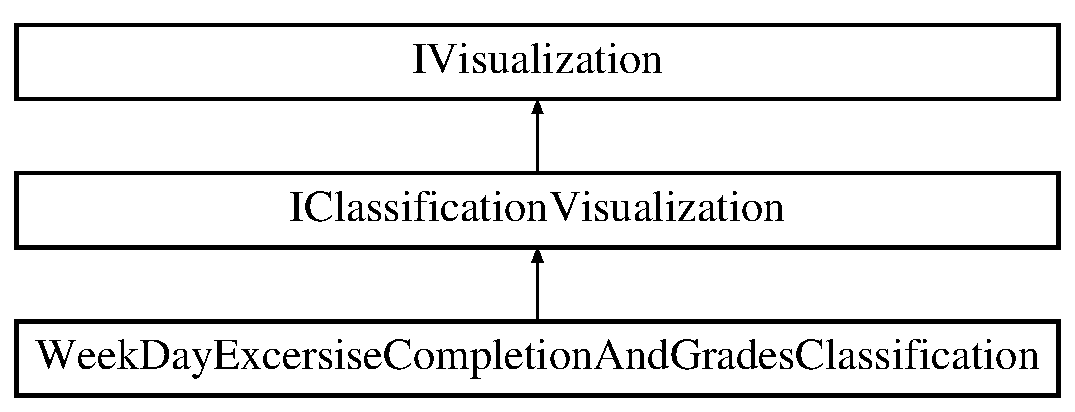
\includegraphics[height=3.000000cm]{classWeekDayExcersiseCompletionAndGradesClassification}
\end{center}
\end{figure}
\subsection*{Public Member Functions}
\begin{DoxyCompactItemize}
\item 
\mbox{\Hypertarget{classWeekDayExcersiseCompletionAndGradesClassification_acb59668b80bf2a80f0697f91ef4bc729}\label{classWeekDayExcersiseCompletionAndGradesClassification_acb59668b80bf2a80f0697f91ef4bc729}} 
{\bfseries Week\+Day\+Excersise\+Completion\+And\+Grades\+Classification} (std\+::shared\+\_\+ptr$<$ \hyperlink{classIClassifier}{I\+Classifier} $>$ cl, std\+::shared\+\_\+ptr$<$ \hyperlink{classIFilter}{I\+Filter} $>$ gf, std\+::shared\+\_\+ptr$<$ \hyperlink{classIFilter}{I\+Filter} $>$ af, std\+::shared\+\_\+ptr$<$ \hyperlink{classITimeFilter}{I\+Time\+Filter} $>$ df, bool filter\+On\+Weekend\+Only)
\end{DoxyCompactItemize}


The documentation for this class was generated from the following files\+:\begin{DoxyCompactItemize}
\item 
Data\+Processer/src/\+Statistical\+Analyzer/\+Visualizations/Week\+Day\+Excersise\+Completion\+And\+Grades\+Classification.\+h\item 
Data\+Processer/src/\+Statistical\+Analyzer/\+Visualizations/Week\+Day\+Excersise\+Completion\+And\+Grades\+Classification.\+cpp\end{DoxyCompactItemize}

\hypertarget{classWeekDayFilter}{}\section{Week\+Day\+Filter Class Reference}
\label{classWeekDayFilter}\index{Week\+Day\+Filter@{Week\+Day\+Filter}}
Inheritance diagram for Week\+Day\+Filter\+:\begin{figure}[H]
\begin{center}
\leavevmode
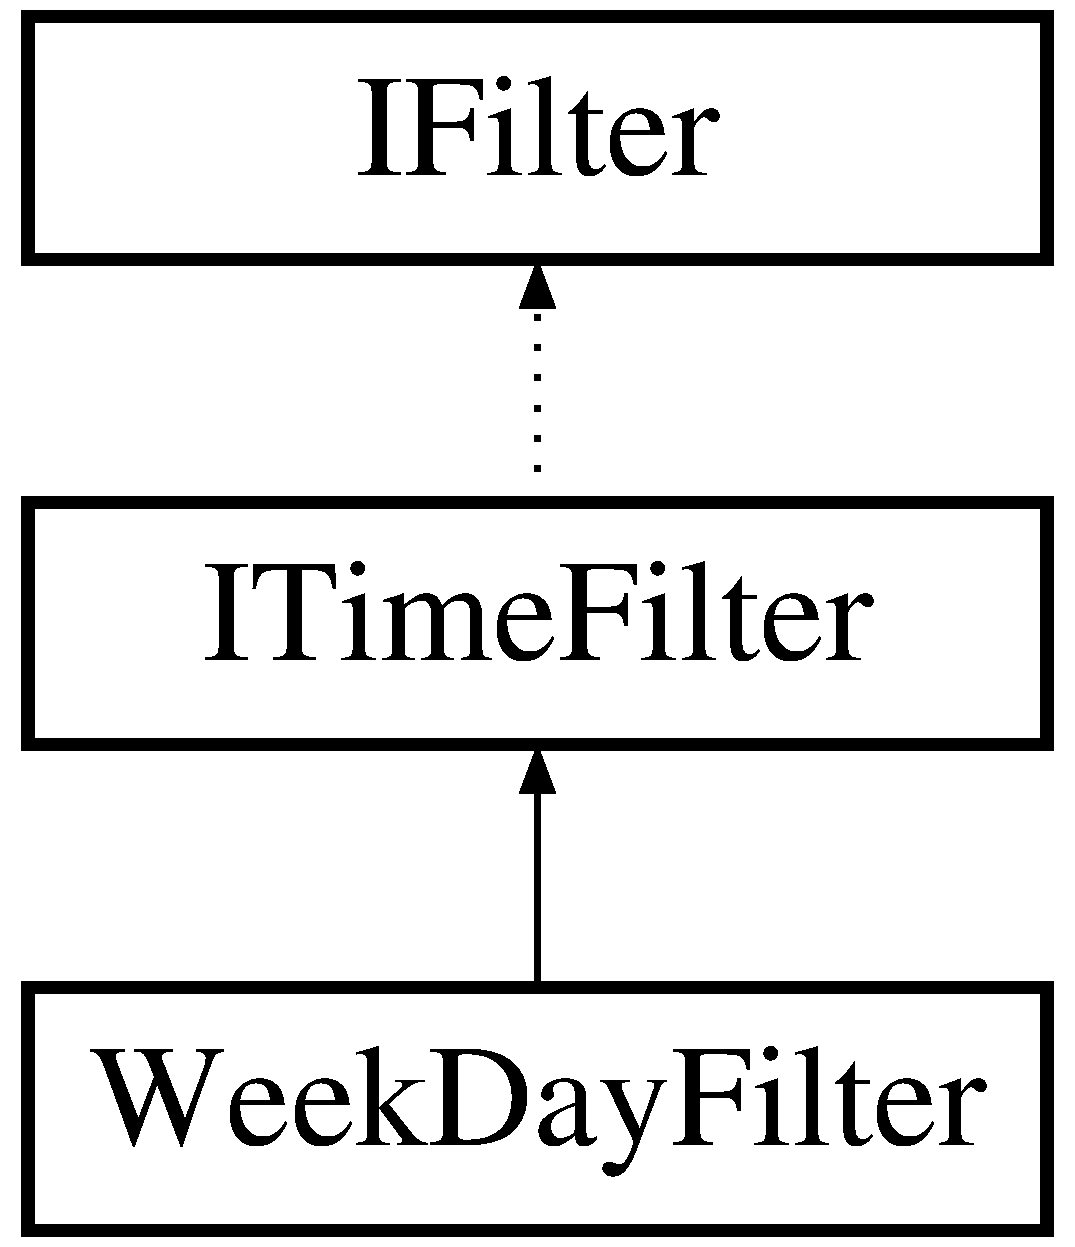
\includegraphics[height=3.000000cm]{classWeekDayFilter}
\end{center}
\end{figure}
\subsection*{Public Member Functions}
\begin{DoxyCompactItemize}
\item 
\mbox{\Hypertarget{classWeekDayFilter_ab0d84d7054d8b84c1d80a8658a5453ff}\label{classWeekDayFilter_ab0d84d7054d8b84c1d80a8658a5453ff}} 
void {\bfseries set\+Filter\+Query\+Column\+Indexes} (\hyperlink{structFilterQueryColumnIndexes}{Filter\+Query\+Column\+Indexes} fq)
\item 
\mbox{\Hypertarget{classWeekDayFilter_a5651f921e2beea0477826404372d8127}\label{classWeekDayFilter_a5651f921e2beea0477826404372d8127}} 
\hyperlink{structFilterQueryColumnIndexes}{Filter\+Query\+Column\+Indexes} {\bfseries get\+Filter\+Query\+Column\+Indexes} ()
\end{DoxyCompactItemize}
\subsection*{Public Attributes}
\begin{DoxyCompactItemize}
\item 
\mbox{\Hypertarget{classWeekDayFilter_a770624363217b22f20fa78d2dacf43e4}\label{classWeekDayFilter_a770624363217b22f20fa78d2dacf43e4}} 
\hyperlink{structFilterQueryColumnIndexes}{Filter\+Query\+Column\+Indexes} {\bfseries query\+Column\+Indexes}
\end{DoxyCompactItemize}


The documentation for this class was generated from the following files\+:\begin{DoxyCompactItemize}
\item 
Data\+Processer/src/\+Statistical\+Analyzer/\+Filter/Week\+Day\+Filter.\+h\item 
Data\+Processer/src/\+Statistical\+Analyzer/\+Filter/Week\+Day\+Filter.\+cpp\end{DoxyCompactItemize}

\hypertarget{classWeekendDayFilter}{}\section{Weekend\+Day\+Filter Class Reference}
\label{classWeekendDayFilter}\index{Weekend\+Day\+Filter@{Weekend\+Day\+Filter}}
Inheritance diagram for Weekend\+Day\+Filter\+:\begin{figure}[H]
\begin{center}
\leavevmode
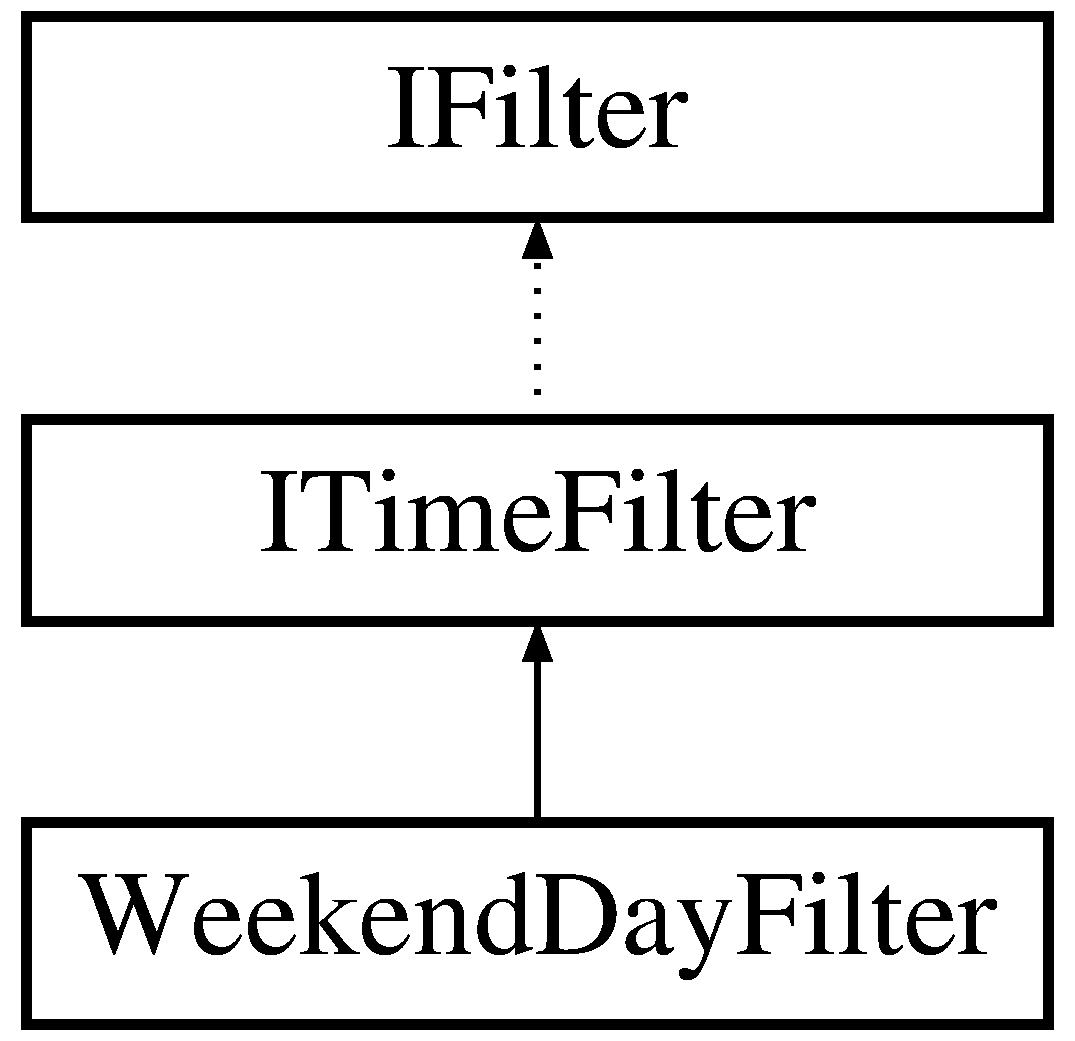
\includegraphics[height=3.000000cm]{classWeekendDayFilter}
\end{center}
\end{figure}
\subsection*{Public Member Functions}
\begin{DoxyCompactItemize}
\item 
\mbox{\Hypertarget{classWeekendDayFilter_a0f6ff3511a2c7bb47e6c22b85810eb4a}\label{classWeekendDayFilter_a0f6ff3511a2c7bb47e6c22b85810eb4a}} 
void {\bfseries set\+Filter\+Query\+Column\+Indexes} (\hyperlink{structFilterQueryColumnIndexes}{Filter\+Query\+Column\+Indexes} fq)
\item 
\mbox{\Hypertarget{classWeekendDayFilter_a86bed8fc0fdb6d5401a9ff45fe2b0794}\label{classWeekendDayFilter_a86bed8fc0fdb6d5401a9ff45fe2b0794}} 
\hyperlink{structFilterQueryColumnIndexes}{Filter\+Query\+Column\+Indexes} {\bfseries get\+Filter\+Query\+Column\+Indexes} ()
\end{DoxyCompactItemize}
\subsection*{Public Attributes}
\begin{DoxyCompactItemize}
\item 
\mbox{\Hypertarget{classWeekendDayFilter_ab632a7f6141066d8b9244850ccb03cf2}\label{classWeekendDayFilter_ab632a7f6141066d8b9244850ccb03cf2}} 
\hyperlink{structFilterQueryColumnIndexes}{Filter\+Query\+Column\+Indexes} {\bfseries query\+Column\+Indexes}
\end{DoxyCompactItemize}


The documentation for this class was generated from the following files\+:\begin{DoxyCompactItemize}
\item 
Data\+Processer/src/\+Statistical\+Analyzer/\+Filter/Weekend\+Day\+Filter.\+h\item 
Data\+Processer/src/\+Statistical\+Analyzer/\+Filter/Weekend\+Day\+Filter.\+cpp\end{DoxyCompactItemize}

\hypertarget{classYamlConverter}{}\section{Yaml\+Converter Class Reference}
\label{classYamlConverter}\index{Yaml\+Converter@{Yaml\+Converter}}
\subsection*{Public Member Functions}
\begin{DoxyCompactItemize}
\item 
\mbox{\Hypertarget{classYamlConverter_a539a4790a7227479dbfc3944d94a6edd}\label{classYamlConverter_a539a4790a7227479dbfc3944d94a6edd}} 
\hyperlink{classYamlObject}{Yaml\+Object} {\bfseries convert\+To\+Basic\+Yaml\+Object} (map$<$ string, string $>$ \&m)
\item 
\mbox{\Hypertarget{classYamlConverter_a020f8eb800db869cfaeaffa3db614a10}\label{classYamlConverter_a020f8eb800db869cfaeaffa3db614a10}} 
void {\bfseries write\+Out\+Yaml\+File} (ofstream \&outfile, vector$<$ \hyperlink{classYamlObject}{Yaml\+Object} $>$ \&yaml\+Objects)
\end{DoxyCompactItemize}
\subsection*{Public Attributes}
\begin{DoxyCompactItemize}
\item 
\mbox{\Hypertarget{classYamlConverter_a0bc3fc92e026b21d4d76e67b01ab3ede}\label{classYamlConverter_a0bc3fc92e026b21d4d76e67b01ab3ede}} 
map$<$ string, string $>$ {\bfseries student\+Ids\+And\+Classes}
\item 
\mbox{\Hypertarget{classYamlConverter_a8f5c802ccb018d8a8e52822a187e7250}\label{classYamlConverter_a8f5c802ccb018d8a8e52822a187e7250}} 
bool {\bfseries generate\+Class\+Hashes}
\item 
\mbox{\Hypertarget{classYamlConverter_ab80f68315a81984cc7220b730f413931}\label{classYamlConverter_ab80f68315a81984cc7220b730f413931}} 
string {\bfseries preferred\+Identifier} = \char`\"{}-\/ id\char`\"{}
\end{DoxyCompactItemize}


The documentation for this class was generated from the following files\+:\begin{DoxyCompactItemize}
\item 
Data\+Processer/src/\+Yaml\+Parser/Yaml\+Converter.\+h\item 
Data\+Processer/src/\+Yaml\+Parser/Yaml\+Converter.\+cpp\end{DoxyCompactItemize}

\hypertarget{classYamlObject}{}\section{Yaml\+Object Class Reference}
\label{classYamlObject}\index{Yaml\+Object@{Yaml\+Object}}
\subsection*{Public Member Functions}
\begin{DoxyCompactItemize}
\item 
\mbox{\Hypertarget{classYamlObject_a9f6674ef3dde95221fd2611654027667}\label{classYamlObject_a9f6674ef3dde95221fd2611654027667}} 
string {\bfseries get\+Identifier} ()
\end{DoxyCompactItemize}
\subsection*{Public Attributes}
\begin{DoxyCompactItemize}
\item 
\mbox{\Hypertarget{classYamlObject_a90d6d602ef87d34c5f827f4d4cad876b}\label{classYamlObject_a90d6d602ef87d34c5f827f4d4cad876b}} 
map$<$ string, string $>$ {\bfseries values}
\item 
\mbox{\Hypertarget{classYamlObject_af6a9b072ca0b39bdfbc34ae4300da3de}\label{classYamlObject_af6a9b072ca0b39bdfbc34ae4300da3de}} 
map$<$ string, \hyperlink{classYamlObject}{Yaml\+Object} $>$ {\bfseries children}
\end{DoxyCompactItemize}
\subsection*{Static Public Attributes}
\begin{DoxyCompactItemize}
\item 
\mbox{\Hypertarget{classYamlObject_a762f87e22e4807a7c0fe0fa117f7c2c1}\label{classYamlObject_a762f87e22e4807a7c0fe0fa117f7c2c1}} 
static string {\bfseries identifier\+Pattern} = \char`\"{}-\/ \char`\"{}
\end{DoxyCompactItemize}


The documentation for this class was generated from the following files\+:\begin{DoxyCompactItemize}
\item 
Data\+Processer/src/\+Yaml\+Parser/Yaml\+Object.\+h\item 
Data\+Processer/src/\+Yaml\+Parser/Yaml\+Object.\+cpp\end{DoxyCompactItemize}

\hypertarget{classYamlParser}{}\section{Yaml\+Parser Class Reference}
\label{classYamlParser}\index{Yaml\+Parser@{Yaml\+Parser}}
\subsection*{Public Member Functions}
\begin{DoxyCompactItemize}
\item 
\mbox{\Hypertarget{classYamlParser_af92bd8a6ba2534b00c685ee66c97a0e8}\label{classYamlParser_af92bd8a6ba2534b00c685ee66c97a0e8}} 
{\bfseries Yaml\+Parser} (ifstream \&filestr)
\item 
\mbox{\Hypertarget{classYamlParser_a8a3bc01ae9a8d5ba769cbc0f4e5e39bb}\label{classYamlParser_a8a3bc01ae9a8d5ba769cbc0f4e5e39bb}} 
vector$<$ \hyperlink{classYamlObject}{Yaml\+Object} $>$ {\bfseries parse\+List\+Of\+Files} (string basefile\+Str)
\item 
\mbox{\Hypertarget{classYamlParser_a83725c913c18c9dd055517978ad9ab86}\label{classYamlParser_a83725c913c18c9dd055517978ad9ab86}} 
vector$<$ \hyperlink{classYamlObject}{Yaml\+Object} $>$ {\bfseries parse\+Yaml} ()
\end{DoxyCompactItemize}
\subsection*{Public Attributes}
\begin{DoxyCompactItemize}
\item 
\mbox{\Hypertarget{classYamlParser_a0aafce56f5c4536636d1e5c9dc603d26}\label{classYamlParser_a0aafce56f5c4536636d1e5c9dc603d26}} 
ifstream \& {\bfseries file}
\end{DoxyCompactItemize}


The documentation for this class was generated from the following files\+:\begin{DoxyCompactItemize}
\item 
Data\+Processer/src/\+Yaml\+Parser/Yaml\+Parser.\+h\item 
Data\+Processer/src/\+Yaml\+Parser/Yaml\+Parser.\+cpp\end{DoxyCompactItemize}

%--- End generated contents ---

% Index
\backmatter
\newpage
\phantomsection
\clearemptydoublepage
\addcontentsline{toc}{chapter}{Index}
\printindex

\end{document}
